% -*- TeX:SI -*-
% slovene sub-mode for spell check
% ----------------------------------------------------------------------
%  Predloga za obliko in navodila za pisanje diplomskih nalog v LaTex-u

%  Univerza v Ljubljani, Fakulteta za elektrotehniko

%  zbral in uredil Roman Kamnik, junij 2013

% ----------------------------------------------------------------------

\documentclass[a4paper,twoside,openright,12pt]{book}
\usepackage[cp1250]{inputenc}  %Kodna stran za Windows okolje, za linux je kodna stran latin2
\usepackage[Slovene]{babel}    % pravila za slovensko deljenje besed
\usepackage[pdftex]{UNI-LJ-FE-Diploma} %Stil za diplome na Fakulteti za elektrotehniko (za pdfTeX v MkiTex)
%\usepackage[pctex]{UNI-LJ-FE-Diploma} %Stil za diplome na Fakulteti za elektrotehniko  (za pcTex)

\usepackage{xkeyval}
\usepackage{graphicx}
\usepackage{epstopdf}
\usepackage{tikz}
\usetikzlibrary{calc}
\usepackage{subcaption} 


\usepackage{hyperref}


\newcommand{\magnet}[5]{% xsredisce, ysredisce, zasuk besedilo v srediscu najb bo crta ali ne
 \pgfmathsetmacro{\Cosa}{cos(#3)}
 \pgfmathsetmacro{\Sina}{sin(#3)}
\draw (#1,#2) circle (2);
\draw (#1+ -2.0 *#5* \Cosa  ,#2 -2.0 *#5* \Sina )--(#1+2.0 *#5* \Cosa , #2+2.0 *#5* \Sina );
\node at (#1-1.6*\Sina ,#2+1.6*\Cosa ){\rotatebox{#3}{N}};
\node at (#1+1.6*\Sina ,#2-1.6*\Cosa  ){\rotatebox{#3}{S}};
\fill (#1,#2) circle [radius=1pt];
}


\newcommand{\senzorja}[4]{% xsredisce, ysredisce, zasuk
 \pgfmathsetmacro{\Cosb}{cos(#3)}
 \pgfmathsetmacro{\Sinb}{sin(#3)}



\hall{#1+2.4*\Cosb }{#2+2.4*\Sinb }{#3}
\hall{#1-2.4*\Sinb}{#2+2.4*\Cosb}{#3}
\fill (#1,#2) circle [radius=1pt];

\draw [dashed, thick](#1,#2)--(#1+2.2*\Cosb ,#2+2.2*\Sinb );
\draw [dashed, thick](#1,#2)--(#1-2.2*\Sinb ,#2+2.2*\Cosb );
}

\newcommand{\hall}[3]{

 \pgfmathsetmacro{\Cosd}{cos(#3)}
 \pgfmathsetmacro{\Sind}{sin(#3)}
 
\draw 
(#1 - 0.2 * \Sind -0.2 * \Cosd  ,#2 + 0.2 * \Cosd -0.2 *\Sind )--
(#1 - 0.2 * \Sind +0.2 * \Cosd  ,#2 + 0.2 * \Cosd +0.2 *\Sind )--
(#1 + 0.2 * \Sind +0.2 * \Cosd  ,#2 - 0.2 * \Cosd +0.2 *\Sind )--
(#1 + 0.2 * \Sind -0.2 * \Cosd  ,#2 - 0.2 * \Cosd -0.2 *\Sind )--
(#1 - 0.2 * \Sind -0.2 * \Cosd  ,#2 + 0.2 * \Cosd -0.2 *\Sind );

\draw (#1-0.1*\Cosd -0.1*\Sind,#2+0.1*\Cosd-0.1*\Sind) --(#1+0.1*\Cosd +0.1*\Sind,#2-0.1*\Cosd+0.1*\Sind);
\draw (#1+0.1*\Cosd -0.1*\Sind,#2+0.1*\Cosd+0.1*\Sind)-- (#1-0.1*\Cosd +0.1*\Sind,#2-0.1*\Cosd-0.1*\Sind);
}
\newcommand{\CaCS}[3]{% razdalja od izhodisca do x max, x komponenta izhodisca, y komponenta izhodisca
	
	\draw [<->](-#1+#2,#3)--(#1+#2,0+#3) node[anchor=north]{$x$};
	\draw [<->](#2,-#1+#3)--(0+#2,#1+#3) node[anchor=east]{$y$};
	
	}

%*************************** PRILAGODITVE *****************************
% mapa s slikami
\potgrafike{./Slike/}
%prilagoditev levega roba sodih strani. �e se pri dvostranskem tisku robovi ne umemajo se lahko pove�a ali pomanj�a
\zamaknirobsodihstrani{0mm}

%*************************** NASLOVNA STRAN *****************************
\naslov{Vpliv stat�ne in dinami�ne ekscentri�nosti na napako senzorja RM44, u�inkovitost kalibracije in robustnost kalibracije na harmonske oscilacije mehanske hitrosti}
\avtor{Mitja Ali�} \univerza{Univerza v Ljubljani}
\fakulteta{Fakulteta za elektrotehniko}
\delo{Magistrsko delo}
%\delo{Diplomsko delo visoko�olskega strokovnega �tudija}
\date{Ljubljana, 2017}
\mentor{doc. dr. Mitja Nemec}
%\somentor{prof. dr. Ime Priimek}
\begin{document}

%------------------------ ZA�ETNI DEL -----------------------------------
%\frontmatter
%%------------------------------------------------------------------------
%
%
%%************************ NASLOVNA STRAN ********************************
%\maketitle
%
%
%%*************************** ZAHVALA ************************************
%\zahvala V zahvali se kandidati zahvali mentorju in poimensko tudi
%vsem sodelavcem in prijateljem, ki so pomagali in prispevali pri
%delu v laboratoriju, na ra�unalniku, v delavnici, pri tehni�ni
%izdelavi dela in drugje.
%
%
%%*************************** VSEBINA *************************************
%\tableofcontents
%
%%*************************** SEZNAM SLIK in TABEL  ***********************
%\seznamslik
%\seznamtabel
%
%%***************************  SEZNAM UPORABLJENIH SIMBOLOV  **************
%
%\seznamsimbolov
%
%V pri�ujo�em zaklju�nem delu so uporabljeni naslednje veli�ine in
%simboli:
%
%\begin{table}[h]
%\centering
%%\begin{footnotesize}
%\begin{tabular}{l l l l}
% \hline \multicolumn{2}{c}{\bf{Veli�ina / oznaka}} & \multicolumn{2}{c}{\bf{Enota}}  \\
% \hline
%Ime & Simbol & Ime & Simbol \\
% \hline
% �as & $t$  & sekunda & s \\
% frekvenca & $f$  & Hertz & Hz \\
% tlak & $p$  & Pascal & Pa \\
% sila vzgona & $\textbf{\textit{f}}_\text{vz}$  & Newton & N \\
% gostota & $\rho$  & - & kg/m$^3$ \\
% masa telesa  & $m_\text{t}$  & kilogram & kg \\
% vhodna napestost & $U_\text{vh}$ & volt  & V \\
% Jacobijeva matrika & $\mathbf{J}$  & - & - \\
%  \hline
%\end{tabular}
%%\end{footnotesize}
%  \caption{Veli�ine in simboli}
%  \label{prebojne_trdnosti}
%\end{table}
%
%
%
%%------------------------ GLAVNI DEL ------------------------------------
%\mainmatter
%%-------------------------------------------------------------------------
%
%
%%********************* POVZETEK V SLOVEN��INI ****************************
%\povzetek
%
%V pri�ujo�em delu so predstavljena navodila za izdelavo 
%
%\kljucnebesede beseda1, beseda2, beseda3
%
%
%%*************************** POVZETEK V ANGLE��INI ***********************
%\abstract
%
%The thesis addresses ...
%
%\keywords word1, word2, word3
%
%
%%***************************** UVOD **************************************
%\chapter{Uvod} \label{uvod}
%
%Uvod v zaklju�no delo ima namen, da uvede bralca v tematiko
%zaklju�nega dela. V njem kandidat raz�leni zahteve in cilje
%zaklju�nega dela, po literaturi povzame znane 
%re"sitve in oceni
%njihov pomen za zaklju�no delo. Sklicevanje na literaturo se v
%besedilu ozna�i s "stevilko v oglatem oklepaju, ki jo ima ta v
%seznamu uporabljenih virov, in po potrebi navede strani, npr.
%\cite{miklavvcivc2010objavljanje} ali \cite[stran 520 -
%534]{juvznivc1992diplomska}.
%
%%*********************** OSREDNJA POGLAVJA ********************************
%\chapter{Izbira teme zaklju�nega dela} \label{izbira_teme}
%
%\chapter{Princip delovanja senzorja RM44}
%
%
%
%
%\chapter{Dolo"canje napake s simulacijo}


\chapter{Uvod}

V dana"snjem "casu elektromotorski pogoni vse hitreje nadome"scajo druge oblike ustvarjanja mehanskega dela. Zahteve po "cim hitrej"si regulaciji in zaneslivosti pogona so "cedalje vi"sje. V pogonih se "zeli dose"ci tudi "cim vi"sji izkoristek. Za doseganje uspe"snega obratovanja elektromotorskega pogona se potrebuje dober in zanesljiv dajalnik pozicije. 
Dejalnike delimo na linearne dajalnike in dajalnike zasuka oz. rotacije. Tu se bom osredoto"cil na rotacijske dajalnike pozicije. Ti so lahko montirani na poljubnem mestu na osi (angl.: through hole), ali le na koncu osi (ang.: On-axis).

%analogni-digitalni senzorji
%relativni absolutni dajalniki

Vsak dajalnik ima to"cnost, katero dose"ze, "ce je pravilno montiran. naapka nepravilne montaze je odvisna od nepravilno postavljenega aktuatorja na osi pogona, ali nepravilno montiranega senzorja. V tem delu bom analiziral kako se napaka ....

V tem delu se bom osredoto"cil na dajalnik RM44, ki ga bom namerno 



Dajalnike lo"cimo tudi glede na uporabljen princip zaznavanja premika. Poznamo magnetne, opti"cne, induktivne in druge. 
Dejalniki se razlikujejo tudi na izodne signale.




\chapter{Dajalniki pozicije RM44}

Dajalnik pozicije RM44 je produkt podjetja RLS merilna tehnika d.o.o. kratica RLS pomeni rotacijski in linearni senzorji zasuka (ang.: Rotary and Linear motion Sensors). Podjetje proizvaja merilnike na podlagi merjenja magnetnega polja. Dajalnik pozicije RM44 spada v dru"zio enkoderjev montiranih na koncu osi rotirajo"ce gredi (ang.: On-axis). Na rotirajo"co os je pritrjen cilindri"cni magnet, ki je diametralno magnetiziran. %(dodaj sliko iz diplome barbare na strani 22 )
Senzor je sestavljen iz "cipa AM8192B, v katerem so vgrajene Hallove sonde za merjenje pravokotne komponente magnetnega polja, magneta montiranega na os pogona. Izhod senzorja je lahko analogen v obliki dveh signalov sinusa in kosinusa. Izhod senzorja je lahko inkrementalni, ki poda relativno spremembo pozicije ter smer premikanja. Senzor lahko prika"ze tudi absolutno vrednost pozicije. Njegova resolucija je nastavljiva med 320 in 8192 pozicij na obrat.

\chapter{Analiti"cna izpeljava dinami"cne in stati"cne eks"centri"cnosti}

Napake so prisotne pravzaprav pri vsakem senzorju. V tem poglavju bom analiti"cno prikazal vpliv napak omenjenih ekscentri"cnosti, ki se pojavijo ob nepravilni monta"zi senzorja. Njuna vpliva ra"zli"cno vplivata na napako zato ju bom obravnaval posami"cno. V delu sem predpostavil, da se izmiki iz idealne pozicije izmikajo le v smeri x in y. Napaka se pojavi tudi ob premiku v smeri z vendar tega tu nebom obravnaval.
 Zaradi narave problema je smiselno uporabiti kartezi"ni koordinatni sistem. V izpeljavah bom predpostavil, da so izmiki majhni. Najprej bom izpeljal po ka"sni trajetoriji se giblje posamezna Hallova sonda. Iz znane tretnutne lokacije Hallove sonde bom lahko izra"cunal vrednost B komponente ki jo meri posamezna Hallova sonda. Pri analiti"cni izpeljavi bom predopstavil, da je polje ob majhnih odmikih linearno in ustreza enacbi polja $B(x,y)=k \cdot y$.  Nato bom analiti"cno izrazil vrednost kota, ki predstavlja izhod senzorja.



\section{Za"cetna pozicija senzorjev}

Za dolo"canje kota med vektorjem ki ka"ze v smeri x-os (\textbf{$1_x$}) in vektorjem med koordinatnim izhodiscem in poljubno to"cko v koordinatnem sistemu, je potrebno poznati poznati le polo"zaj to"cke. Primer je podan na sliki \ref{fig:dolocitev_kota}. Kot $\varphi$ dolo"cimo preko trigonometri"cne funkcije $\arctan$: $$\varphi=\arctan\frac{y_0}{x_0}$$



\begin{figure}[h!]
	\centering
	\begin{tikzpicture}[scale=4]
	\CaCS{0.75}{0}{0}
	\draw [->,thick](0,0)--(-0.5,0.2855);
	\draw (0.15,0) arc (0:150:0.15);
	\node at (0.05,0.05){$\varphi$};
%	\node at (-0.5,0.285) {\textbullet};
	\node at (-0.32,0.35) {($x_0$,$y_0$)};
	\end{tikzpicture}
	\caption{Slika za pomo"c pri dolo"canju kota}
	\label{fig:dolocitev_kota}
\end{figure}


Za dolo"citev kota $\varphi$  je dovolj poznati "ze projekciji vektorja na koordinatni osi(slika \ref{fig:dolocitev_kota_2}),

\begin{figure}[h!]
	\centering
	\begin{tikzpicture}[scale=4]
	\CaCS{0.75}{0}{0}
	\draw [->,thick](0,0)--(-0.5,0.2855);
	\draw (0.15,0) arc (0:150:0.15);
	\node at (0.05,0.05){$\varphi$};
	\draw [dashed] (-0.5,0.2855)--(-0.5,0);
	\draw [dashed] (-0.5,0.2855)--(0,0.2855);
	%	\node at (-0.5,0.285) {\textbullet};
%	\node at (-0.32,0.35) {($x_0$,$y_0$)};
	\node at(-0.5,-0.1){$x_0$} ;
	\node at(0.1,0.2855){$y_0$};
	\end{tikzpicture}
	\caption{Slika za pomo"c pri dolo"canju kota}
	\label{fig:dolocitev_kota_2}
\end{figure}


"Ce poznamo le projekciji to"cke na koordinatni osi, je to zadosten pogoj za dolo"citev kota $\varphi$.
Za dolo"citev kota zasuka v idealnih pogojih, kot je predpostavka, da je polje linearno, sta dovolj dve Hallovi sondi, ki sta prostorsko zamaknjeni za 90$^\circ$ (Slika \ref{fig:zacetna_postavitev_sond}).

Za"cetni lokaciji sond enostavmo postavimo na koordinatni osi in s tem ustre"zemo pogoju po prostorskem zasuku med sondama. Sondi postavimo na razdaljo $r_0$ od koordinatnega izhodi"s"ca. S tem dobimo za"cetni lokaciji Hallovih sond $\mathrm{H}_1(x_0, y_0)=(r_0, 0)$, $\mathrm{H}_2(x_0, y_0)=(0, r_0)$.



\begin{figure}[h!]
	\centering
	\begin{tikzpicture}[scale=1]
	\CaCS{3}{0}{0}
	\senzorja{0}{0}{0}{}
%	\magnet {0} {0} {10}{ }{0}
	\node at (2.0,-0.5){$\mathrm{H}_1(r_0,0)$};
	\node at (-1,2.3){$\mathrm{H}_2(0, r_0)$};
	\end{tikzpicture}
	\caption{Za"cetna postavitev Hallovih sond}
	\label{fig:zacetna_postavitev_sond}
\end{figure}


\section{Zasuk magneta}

Z zasukom magneta za kot $\theta$ se na mestu, kjer merimo magnetno polje, polje spremni. Polje bi se spremnilo enako "ce bi nad magnetom  zasukali senzor za kot $-\theta$. Hallova sonda z za"cetno lokacijo ($x_0, y_0$) bi se po kro"znici premaknila v novo lokacijo($\mathrm{x, y}$):
\begin{equation}
\label{eq:osnovni_zasuk}
\begin{bmatrix}
x\\y
\end{bmatrix}= \begin{bmatrix}
\cos (-\theta)& -\sin(-\theta)\\ \sin( -\theta)& \cos (-\theta)
\end{bmatrix}
\cdot
\begin{bmatrix}
r_0\\r_0
\end{bmatrix}
\end{equation}
Z upo"stevanjem da je funkcija sinus liha in funkcija kosinus soda, se izra"cun v ena"cbi \ref{eq:osnovni_zasuk} poenostavi v:
\begin{equation}
\label{eq:osnovni_zasuk_popravljena_rot}
\begin{bmatrix}
x\\y
\end{bmatrix}= \begin{bmatrix}
\cos (\theta)& \sin(\theta)\\ -\sin( \theta)& \cos (\theta)
\end{bmatrix}
\cdot
\begin{bmatrix}
r_0\\r_0
\end{bmatrix}
\end{equation}




\begin{figure}[h!]
	\begin{subfigure}[b]{0.5\textwidth}
		\centering
		
		\resizebox{\linewidth}{!}{
			\begin{tikzpicture}
	\senzorja{0}{0}{0}{ }
	\magnet {0} {0} {-60}{ }{1}

	\draw (1.2,0) arc (0:30:1.2) node at (0.8,0.2){$\theta$}[dashed]--(0,0);
			\end{tikzpicture}
		}
		
		\caption{Zasukan magnet za kot $\mathrm{\theta}$}
		\label{fig:subfig8}
	\end{subfigure}
	\begin{subfigure}[b]{0.5\textwidth}
		\centering
		\resizebox{\linewidth}{!}{
			\begin{tikzpicture}

				\senzorja{0}{0}{-30}{ }
				\magnet {0} {0} {-90}{ }{1}
				\draw [dashed](0,0)--(1.2,0) arc (0:-30:1.2);
				\node at (0.9,-0.25){$-\theta$};
			\end{tikzpicture}
		}
		\caption{Zasukan senzor za kot $\mathrm{-\theta}$}   
		\label{fig:subfig9}
	\end{subfigure}

	\caption{Hallovi sondi se glede na magnet nahajati na enaki lokaciji}
	\label{fig:subfig1.a.4}
\end{figure}




Ko zavrtimo senzor okoli magneta pri tem pomeri polje. Ker sem predpostavil linearno polje, ga predstavim s izrazom 
\begin{equation}
\label{eq:enacba_polja}
B(x,y)=k \cdot x
\end{equation}
Za poenostavitev vzemimo $k=1$. S tem se ena"cba \ref{eq:enacba_polja} poenostavi v:
\begin{equation}
\label{eq:enacba_polja_2}
B(x,y)=x
\end{equation}


Polje ki ga pomeri posamezna sonda dobimo z upostevanjem ena"cb \ref{eq:osnovni_zasuk_popravljena_rot} in \ref{eq:enacba_polja_2}.
\begin{equation}
B_{H_1}(\theta)=r_0\cdot \sin \theta
\end{equation}
\begin{equation}
B_{H_2}(\theta)=r_0\cdot \cos \theta
\end{equation}

\slikaeps{Magnetno polje, ki ga pomeriti sondi, ko je monta"za pravilna}{B1B2_brez_eks}% ob sliki pise s katerim programom jo generiras: vrednost_polja_real.m r0=1


\section{Izpeljava ena"cb pri dinami"cni ekscentri"cnosti}

%Zaradi splo"snosti predpostavimo da sta sredi"s"ci v za"cetni legi poravnani vendar je magnet glede na senzor zasukan za kot $\lambda$ (Slika \ref{fig:definicija_lambde}).  Ta je v primeru ko je smer poravnana z za"cetno lego magneta enaka 0. V nasprotnem primeru pa kot upo"stevamo v definiciji njene lege glede na kot magneta $\theta -\lambda$.  Ta zasuk bo imel na obe Hallovi sondi enak vpliv. Zato si lahko privo"s"cimo implementacijo kota  $\lambda$, ki temelji na principu superpozicije. 
%
%
%\begin{figure}[h!]
%	\centering
%	
%	\begin{tikzpicture}
%	\senzorja{0}{0}{0}{ }
%	\magnet {0} {0} {-60}{ }{1}
%	
%	\draw[dashed](0.0,0)--(1.5,0)arc(0:30:1.5)--(0.,0);
%	\node at (1.2,0.3){$\lambda$};
%	
%	\end{tikzpicture}
%	
%	\caption{Zasukan magnet za kot $\mathrm{\theta}$}
%	\label{fig:definicija_lambde}
%	
%\end{figure}
Opazujmo sedaj opisan sistem z dodano dinami"cno ekscentri"cnostjo. Definirajmo za"cetno lego rotorja v centru statorja $S_r(0, 0)=S_s(0, 0)$. Rotor izmaknemo iz za"cetne lege v novo sredi"s"ce $S_r(\Delta x_d, \Delta y_d,)$. Os vrtenja ostaja v centru statorja, zato staro sredi"s"ce rotorja opisuje kro"znico s polmerom $\sqrt{\Delta x_d^2+ \Delta y_d^2}$. 






\begin{figure}[h!]
	\begin{subfigure}[b]{0.5\textwidth}
		\centering
		\resizebox{\linewidth}{!}{
			\begin{tikzpicture}
	\senzorja{0}{0}{0}{$S_s(0, 0)$}
	\magnet {0.5} {0.5} {-30}{$S_r(\Delta x_d, \Delta y_d)$}{1}
	\draw [dotted,thick](0,0) circle [radius=0.707];
	\draw [dashed](1.5,0) arc (0:30:1.5)--(0,0);
	\node at(1,0.3){$\theta$};
			\end{tikzpicture}
		}
		\caption{Zasukan magnet za kot $\mathrm{\theta}$}
		\label{fig:teorija_dinamika_1}
	\end{subfigure}
	\begin{subfigure}[b]{0.5\textwidth}
		\centering
		\resizebox{\linewidth}{!}{
			\begin{tikzpicture}
	\senzorja{-0.5}{-0.5}{-30}{$S_s(-\Delta x_d, -\Delta y_d)$}
	\magnet {0} {0} {-90}{$S_r(0, 0)$}{1}
	\draw [dotted, thick](-0.5, -0.5) circle [radius=2.4];
	
	\draw  [dashed](-0.5,-0.5)--(1,-0.5) arc (0:-30:1.5);
	\node at (0.5, -0.75){$-\theta$};
			\end{tikzpicture}
		}
		\caption{Zasukan senzor za kot $\mathrm{-\theta}$}   
		\label{fig:teorija_dinamika_2}
	\end{subfigure}ub
	
	\caption{Hallovi sondi se glede na magnet nahajati na enaki lokaciji}
	\label{fig:subfig1.a.4}
\end{figure}




"Ce sedaj sistem miselno obrnemo kot sem to napravil v prej"njem poglavju in senzor zavrtimo. Ob takem premiku senzor opi"se trajektorijo kot pri pravilno montiranem senzorju le z dodano translacijo ekscentri"cnosti. Kako Hallova sonda spreminja lokacijo glede na vrtenje je prikazano na sliki \ref{fig:teorija_dinamika_2}, s pik"casto kro"znico.


Novo lokacijo Hallove sonde lahko dolo"cimo po ena"cbi \ref{eq:dinamicna_ekscentricnost}.
\begin{equation}
\label{eq:dinamicna_ekscentricnost}
\begin{bmatrix}
x\\y
\end{bmatrix}= \begin{bmatrix}
\cos (\theta)& \sin(\theta)\\ -\sin( \theta)& \cos (\theta)
\end{bmatrix}
\cdot
\begin{bmatrix}
r_0\\r_0
\end{bmatrix}
+
\begin{bmatrix}
-\Delta x_d \\ -\Delta y_d
\end{bmatrix}
\end{equation}
Ena"cbo \ref{eq:dinamicna_ekscentricnost} lahko poenostavimo pri "cemer $\Delta x_d$ in $\Delta y_d$ predstavlja vrednost za koliko je rotor izmaknjen iz osi vrtenja.
\begin{equation}
\label{eq:dinamicna_ekscentricnost_popravljena}
\begin{bmatrix}
x\\y
\end{bmatrix}= \begin{bmatrix}
\cos (\theta)& \sin(\theta)\\ -\sin( \theta)& \cos (\theta)
\end{bmatrix}
\cdot
\begin{bmatrix}
r_0\\r_0
\end{bmatrix}
-
\begin{bmatrix}
\Delta x_d \\ \Delta y_d
\end{bmatrix}
\end{equation}

Z upo"stevanjem magnetnega polja po izrazu \ref{eq:enacba_polja_2} izrazimo odvistnost magnetnega polja od kota zasuke in ekscenri"cnosti. Iz potekov magnetnega polja v izrazih (\ref{eq:B_H_1_dinamicen}) in (\ref{eq:B_H_2_dinamicen}) opazimo da magnetno polje ni odvisno od dinami"cne eks"centri"cnosti v y smeri. S hitrim miselnim eksperimentom si lahko hitro predstavljamo, da "ce senzor izmaknemo v smeri y magnetno polje na novi lokaciji ostane enako. 

\begin{equation}
\label{eq:B_H_1_dinamicen}
B_{H_1}(\theta)=r_0\cdot \cos \theta -\Delta x_d
\end{equation}
\begin{equation}
\label{eq:B_H_2_dinamicen}
B_{H_2}(\theta)=r_0\cdot \sin \theta-\Delta x_d
\end{equation}



\slikaeps{Magnetno polje, ki ga pomeriti sondi, ko je magnet izmaknjen}{B1B2_din_eks}%vrednost_polja_real.m





\section{Izpeljava ena"cb pri stati"cni ekscentri"cnosti}

Opazovani sistem ostaja enak, brez ekscentri"cnosti. Sedaj iz osi vrtenja izmaknemo senzor. Os magneta in os vrtenja sta poravnani.  Sredi"s"ce senzorja se sedaj nahaja na koorinatah $S_s(\Delta x_s, \Delta y_s)$. kot pri izpeljavi pri dinami"cni ekscentri"cnosti obrnimo sistem in zavrtimo senzor upo"stevajo"ce z ekscentri"cnostjo. Sredi"s"ce senzorja opi"se kro"znico okoli sredi"sca magneta oz. osi vrtenja. Hallovi sondi se vrtita vsaka po svoji kro"znici. Gibanje posamezne sonde lahko opi"semo z izrazom:

   \begin{equation}
   \label{eq:dinamicna_ekscentricnost_popravljena}
   \begin{bmatrix}
   x\\y
   \end{bmatrix}=
   \begin{bmatrix}
   \cos (\theta)& \sin(\theta)\\ -\sin( \theta)& \cos (\theta)
   \end{bmatrix}
   \cdot
   \begin{bmatrix}
   r_0+\Delta x_s\\r_0+\Delta y_s
   \end{bmatrix}
   \end{equation}

Magnetno polje, ki ga pomerita dobimo iz izraza (\ref{eq:enacba_polja_2}).

\begin{equation}
\label{eq:B_H_1_staticen}
B_{H_1}=(r_0+\Delta x_s)\cos(\theta)+\Delta y_s \sin(\theta)
\end{equation}
\begin{equation}
\label{eq:B_H_2_staticen}
B_{H_1}=-\Delta x_s\sin(\theta)+(r_0+\Delta y_s) \cos(\theta)
\end{equation}













\begin{figure}[h!]
	\begin{subfigure}[b]{0.5\textwidth}
		\centering
		\resizebox{\linewidth}{!}{
			\begin{tikzpicture}
			\senzorja{0.5}{-0.5}{0}{$S_s(\Delta x_s, \Delta y_s)$}
			\magnet {0} {0} {-60}{$S_r(0, 0)$}{1}
		
		
			\node at (0.75,-0.75){$S_s(\Delta x_s, \Delta y_s)$};
			\node at (-0.75,0){$S_r(0, 0)$};
			
		
			\draw [dashed](0,0)--(1.6,0) arc (0:30:1.6)--(0,0);
			\node at(1,0.3){$\theta$};
			

			
			\end{tikzpicture}
		}
		\caption{Zasukan magnet za kot $\mathrm{\theta}$ in statina eksenri"cnost}
		\label{fig:teorija_statika_1}
	\end{subfigure}
	\begin{subfigure}[b]{0.5\textwidth}
		\centering
		\resizebox{\linewidth}{!}{
			\begin{tikzpicture}
%			\senzorja{0.5}{-0.5}{0}{$S_s(-\Delta x_d, -\Delta y_d)$}
			\senzorja{0.183}{-0.683}{-30}{$S_s(-\Delta x_d, -\Delta y_d)$}
			\magnet {0} {0} {-90}{$S_r(0, 0)$}{1}


			\draw [dashed](0,0)--(1.5,0) arc (0:-30:1.5)--(0,0);
			\node at(1.1,-0.3){$-\theta$};


			
			
			\draw [dotted](0,0) circle [radius=0.707];
		
%			\node at (0,-1){$S_s(\Delta x_s, \Delta y_s)$};
			\node at (-0.22,0.25){$S_r(0, 0)$};			
		
     			\draw [dotted](0,0) circle	[radius=2.94];
     			\draw [dotted](0,0) circle	[radius=1.965];
     		                                                                                     
			\end{tikzpicture}
		}
		\caption{Zasukan senzor za kot $\mathrm{-\theta}$}   
		\label{fig:teorija_statika_2}
	\end{subfigure}ub
	
	\caption{Hallovi sondi se glede na magnet nahajati na enaki lokaciji}
	\label{fig:subfig1.a.4}
\end{figure}




\slikaeps{Magnetno polje, ki ga pomeriti sondi, ko je senzor izmaknjen}{B1B2_sta_eks}%vrednost_polja_real.m


\section{Kon"cna ena"cba za dolo"citev lokacije sonde in dolo"canje pomerjenega kota}


Sedaj lahko izraza za dolo"canje lokacije in hkrati magnetnega polja zapi"semo z eno ena"cbo:



   \begin{equation}
   \label{eq:enacba_lokacije}
   \begin{bmatrix}
   x\\y
   \end{bmatrix}=
   \begin{bmatrix}
   \cos (\theta)& \sin(\theta)\\ -\sin( \theta)& \cos (\theta)
   \end{bmatrix}
   \cdot
   \begin{bmatrix}
   x_0+\Delta x_s\\y_0+\Delta y_s
   \end{bmatrix}
   -
   \begin{bmatrix}
   \Delta x_d\\ \Delta y_d
   \end{bmatrix}
   \end{equation}

Polje ki ga opi"seti sondi se glasi:
\begin{equation}
\label{B_H_1_koncna}
B_{H_1}=(r_0+\Delta x_s) \cos(\theta)+\Delta y_s \sin(\theta)-\Delta x_d
\end{equation}
\begin{equation}
\label{B_H_2_koncna}
B_{H_2}=\Delta x_s \cos(\theta)+(r_0+\Delta y_s) \sin(\theta)-\Delta x_d
\end{equation}

Iz izrazov (\ref{B_H_1_koncna}) in (\ref{B_H_2_koncna}) sedaj lahko izra"cunamo kot.

\begin{equation}
\label{eq:dolocanje_kota_splosna}
\varphi=\arctan \frac{B_{H_2}}{B_{H_1}}
	=\arctan \frac{\Delta x_s \cos(\theta)+(r_0+\Delta y_s) \sin(\theta)-\Delta x_d}
	{(r_0+\Delta x_s) \cos(\theta)+\Delta y_s \sin(\theta)-\Delta x_d}
\end{equation}


%https://dspguru.com/files/Sum_of_Two_Sinusoids.pdf vir za izracun trigonometrije


%http://ieeexplore.ieee.org/stamp/stamp.jsp?arnumber=6375931
%http://ieeexplore.ieee.org/stamp/stamp.jsp?arnumber=6567733
%http://ieeexplore.ieee.org/stamp/stamp.jsp?arnumber=4054743
%http://ieeexplore.ieee.org/stamp/stamp.jsp?arnumber=5346438
%http://www.embedded.com/design/other/4216719/Performing-efficient-arctangent-approximation
%

%Zaradi majhnih odmikov lahko predpostavim, da je pravokotna komponenta vektorja gostote magnetnega pretoka(vektor \textbf{B}) linearna. S tem se izpeljava za dolo"canje pozicije, poenostavi. Kasneje bom predstavil tudi na"cin kako pridobiti vredn ost \textbf{B} realnega polja. Predpostavil bom tudi da je senzor za mejenje pozicije sestavljen le iz dveh Hallovih sond, pri kateri je druga sonda fazno premaknjena za 90$^\circ$. 
%slika kjer je narisano linearno polje

\section{Dolo"canje kota pri stati"cni ekscntri"cnosti v smeri x }

Zaradi nelinearnosti fukcije $\arctan$ je izraz (\ref{eq:dolocanje_kota_splosna}) analiti"cno te"zko poenostaviti v polni obliki. Zato se vsake ekscentri"cnosti lotim posami"cno. "Ce upo"stevamo le ekscentri"cnost $\Delta x_s$ se izraz (\ref{eq:dolocanje_kota_splosna}) poenostavi v:
\begin{equation}
\label{eq:dolocanje_kota_xs}
\varphi=
\arctan \frac{\Delta x_s \cos(\theta)+r_0 \sin(\theta)}
{(r_0+\Delta x_s) \cos(\theta)}
\end{equation}


Z upo"stevanjem Taylorjeve vrse za $\arctan$:
\begin{equation}
\arctan(x)=x-\frac{x^3}{3}... pri |x|\leq 1
\end{equation}

Izraz lahko zapi"semo kot

\begin{equation}
\varphi=  \frac{\Delta x_s \cos(\theta)+r_0 \sin(\theta)}
{(r_0+\Delta x_s) \cos(\theta)}+
\frac{(\Delta x_s \cos(\theta)+r_0 \sin(\theta))^3}
{3((r_0+\Delta x_s) \cos(\theta))^3}
\end{equation}



\section{Dolo"canje pribli"zka za funkcijo $\arctan$}

Funkcija arkustangens ($\arctan$), je inverzna funkcija funkcije tangens.

Zaloga vrednosti je v obmo"cju med $-\pi/2$ in $\pi/2$. Funkcija arkustangens tako zajame le polovico periode. V numeriki se za dolo"citev kota na celi periodi
 $[-\pi, \pi]$ uporablja funkcijo $atan2$, ki sprejme dva parametra in na podlagi njunih predznakov dolo"ci v katerem kvadrantu se nahaja iskani kot. 
 
 \[
 \varphi=atan2(x,y)=
 \begin{cases}
 [0, \frac{\pi}{2}]:&  x\geq 0, y\geq 0 \\
 [\frac{\pi}{2}, \pi]:& x\leq 0, y\geq 0\\
 [-\pi, -\frac{\pi}{2}]:& x\leq 0, y\leq 0\\
 [-\frac{\pi}{2}, 0]:& x\geq 0, y\leq 0
 \end{cases}
 \]




Funkcija $atan2$ nato preko funkcije $\arctan$ izra"cuna vrednost na podlagi razmerja $\frac{y}{x}$. Iz izraza (\ref{eq:arctan_picetrt}) lahko vidimo, da je potrebno poznati za funkcijo $\arctan$ zalogo vrednosti le med $-\frac{\pi}{4}$ in $\frac{\pi}{4}$. 
 \begin{equation}
\label{eq:arctan_picetrt}
 \arctan x=\frac{\pi}{2}-\arctan \frac{1}{x}
\end{equation}

Za dolo"citev kota ne glede kje na periodi, je potrebno izra"cunati kvocient med spremenljivko x in y. Da bi se izognil temu deljenju sem aproksimiral funkcijo $f(x,y)=\arctan(\frac{y}{x})$ z ravnino (\ref{eq:polinom}).
\begin{equation}
\label{eq:polinom}
\varphi(x,y)=a_1 x^3 + a_2 x^2 y + a_3 x^2 + a_4 x y^2 + a_5 x y + a_6 x + a_7 y^3 + a_8 y^2 + a_9 y + a_{10}
\end{equation}

Funkcijo sem aproksimiral na naklju"cno razporejene to"cke po "cetrtini kro"znega  kolobarja $\varphi \in [-\frac{\pi}{4}, \frac{\pi}{4}]$, z radijema $a=r_0-0.2$~mm in $b=r_0+0.2$~mm.



\begin{figure}[!h]
	\label{fig:obmocje_tock}
	\centering
	\begin{tikzpicture}
	\draw [<->](-1,0)--(3,0) node[anchor=north]{$x$};
	\draw [<->](0,-2.5)--(0,2.5) node[anchor=east]{$y$};
	\fill [blue] (1.5556*0.9,-1.5556*0.9) arc (-45:45:2.2*0.9)--(1.0*1.8385,1.0*1.8385)arc (45:-45:1.0*2.6)--(1.5556*0.9,-1.5556*0.9);
		\end{tikzpicture}
		\caption{Obmo"cje nahajanja akljucnih to"ck}
\end{figure}

Za to"cke znotraj obmo"cja sem izracunal vrednost $\arctan \frac{y}{x}$. Na to sem z uporabo funkcije polyfitn(dodaj vir), aproksimiral ravnino definirano z izrazom (\ref{eq:polinom}). Dobil sem koeficiente katere sem lahko uporabil v izra"cunih za analiti"cen prikaz napake. Ravnina je na definiranem obmo"cju odstopala za najve"c $0,253^\circ$. S predpostavko, da bo napaka ob dovolj veliki ekscentri"cnosti, vi"sja od napake zaradi aproksimacije ravnine sem v izraz za ravnino, vstavil izraza (\ref{B_H_1_koncna}) in(\ref{B_H_2_koncna}). Izpeljava je prikazana v dodatku. Izrazi se poenostavijo "ce posami"cno obravnavam vsako ekcentri"cnost. 

Z vnosom "stevilk sej je pokazalo, da bo pri stati"cnem izmiku nekoliko bolj izrazit drugi harmonik napake, kot pri dinami"cni ekscentri"cnosti. 

Tu se kaj napisati

Ve"c informacij je bilo te"zko izlu"sciti, saj je bila funkcija $\arctan$ aproksimirana z ravnino dveh spremenljivk le na "cetrtini celotne periode.

\chapter{Numeri"cen izra"cun napake}

Od tu naprej sem za izra"cun kota uporabljal vgrajeno funkcijo $atan2$, ki numeri"cno dolo"ci izhodni kot $\varphi$ glede na vhodni spremenljivki x in y. Pri izra"cunih sem postavil hallovi sondi na razdaljo $r_0=2,4$~mm, vsako ekscentri"cnost posamezno  sem simuliral z $0,1$~mm izmikom.

\subsection{Napaka pri stati"cni ekscentri"cnosti v smeri x-osi}

Z vnosom izrazov (\ref{B_H_1_koncna}) in (\ref{B_H_2_koncna}) v funkcijo $atan2$, s stati"cno ekscentri"cnostjo v x-osi se pojavi napaka definirana kot 
\begin{equation}
\varepsilon= \varphi - \theta
\end{equation}


  \begin{figure}[h!]
  	\begin{center}
  		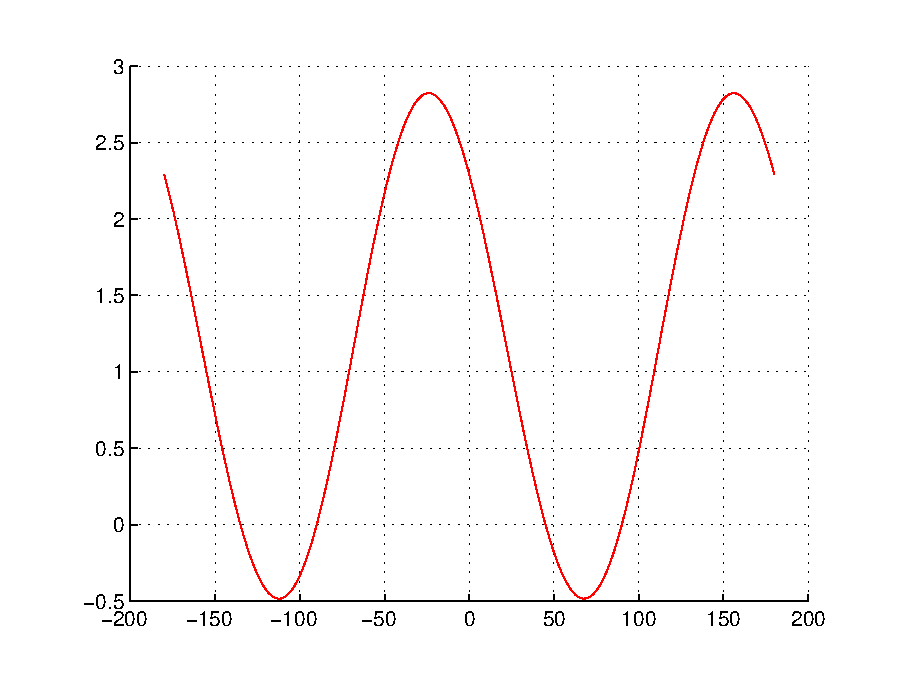
\includegraphics[scale=0.5]{\dirslike/protokol_xs_1.eps}%vrednost_polja_real.m nastavis r0 na 2.4
  	\end{center}
  	\caption{numericen izracun napake}
  	\label{fig:protokol_xs_1}
  \end{figure}

Iz slike \ref{fig:protokol_xs_1} se vidi napaka v obliki enosmerne komponente in drugega harminika na periodo. Napaka se s konstantnim vrtenjem magneta ne akumulira, zato je dovolj prikaz napake na eni periodi. Napako razvijem v Fouriejevo vrsto do osmega harmonika. Amplitude posameznih harmonikov za stati"cno ekscentri"cnost v smeri x osi za izmik $0,1$~mm so prikazane na sliki \ref{fig:vrsta_protokola_xs_1}.

\begin{figure}[h!]

	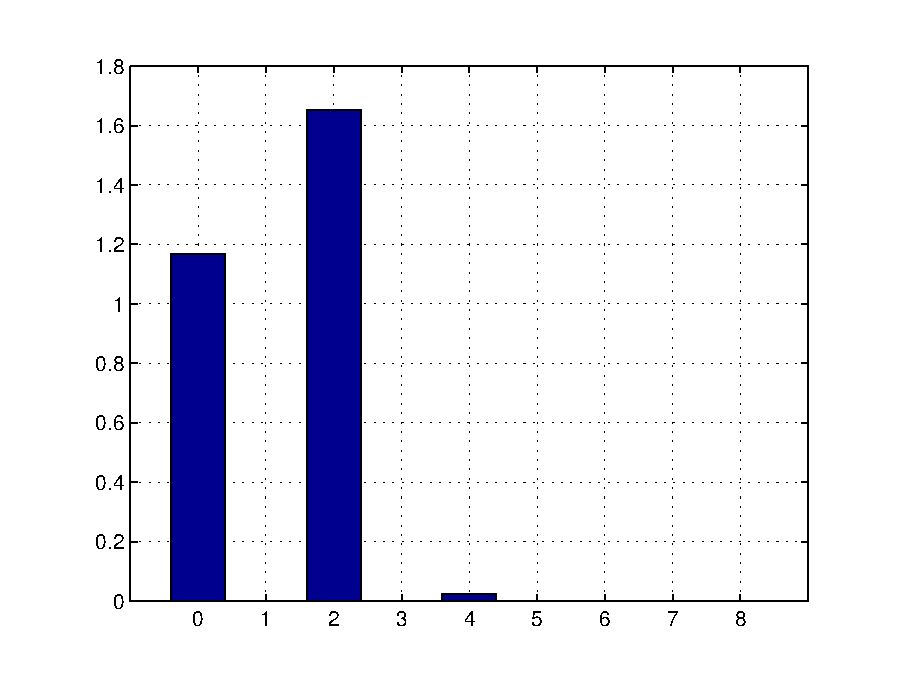
\includegraphics[scale=0.7]{\dirslike/vrsta_protokola_xs_1}%vrednost_polja_real.m narisanih 8 harmonikov
	\caption{AAmplitude harmonikov protokola}
	\label{fig:vrsta_protokola_xs_1}
\end{figure}


Kot smo "ze predpostavili po sliki \ref{fig:protokol_xs_1} izstopata predvsem enosmerna komponenta in drugi harmonik. Nakaj je "se "cetrtega harmonika medtem ko so ostali harmoniki zanemarljivi.



\subsection{Napaka pri stati"cni ekscentri"cnosti v smeri y-osi}


Pri stati"cni ekscentri"cnosti sem ponovil postopek kot pri stati"cni ekscentri"cnosti v smeri x-osi. Pri"cakoval sem podobene rezultate, kot pri stati"cni ekscentri"cnosti v smeri x-osi. Napaka kota $\varepsilon$ je prikazana na sliki \ref{fig:protokol_ys_1}. Prav tako kot pri napaki ob stati"cni ekscentri"cnosti v smeri x-osi izstopa enosmerna komponenta in drugi harmonik. Opazimo, da je enosmerna komponenta spremenila predznak. Iz Fouriejeve vrste (slika \ref{fig:vrsta_protokola_ys_1}) Opazimo rezultate podobne kot pri stati"cni ekscentri"cnosti v smeri x-osi. Izstopajo enosmerna komponenta drugi harmonik, obstaja tudi "cetrti harmonik, ostali so zanemarljivi. 
Zanimivost lahko razberemo "se iz faznega premika. Napaka pri stati"cni ekscentri"cnosti v smeri y-osi, za stati"cno napako v smeri x-osi, fazno zaostaja ravno za velikost dveh faznih kotov. To se pojavi pri drugem in "sestem harmoniku. "sesti harmonik je po amplitudi zanemarljiv zato je zanimiv podatek o faznem kotu le za drugi harmonik.


  \begin{figure}[h!]
  	\begin{center}
  		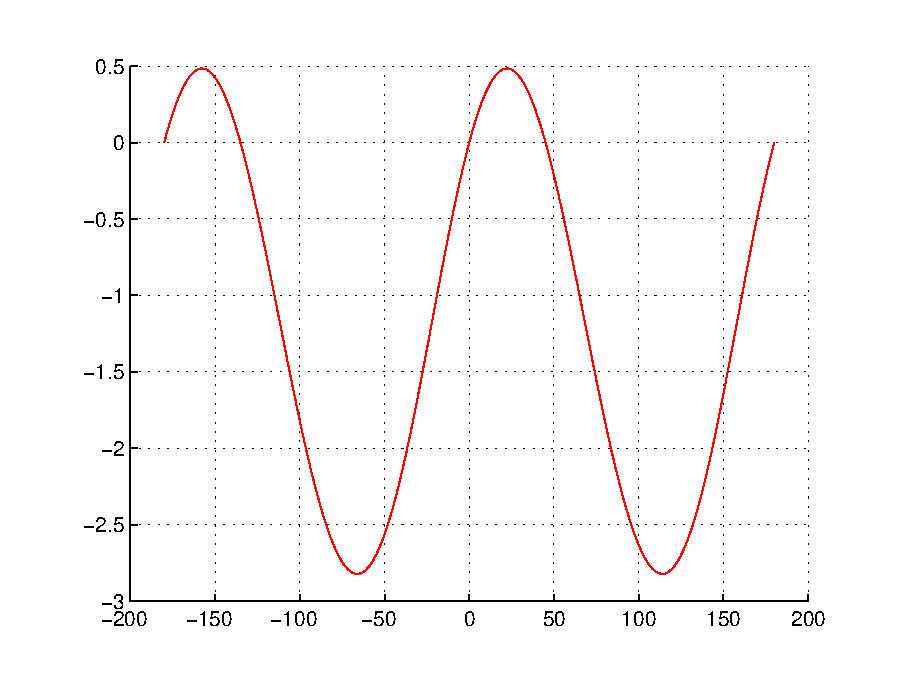
\includegraphics[scale=0.5]{\dirslike/protokol_ys_1.eps} %vrednost_polja_real.m
  	\end{center}
  	\caption{numericen izracun napake}
  	\label{fig:protokol_ys_1}
  \end{figure}
  
  
\begin{figure}
	
	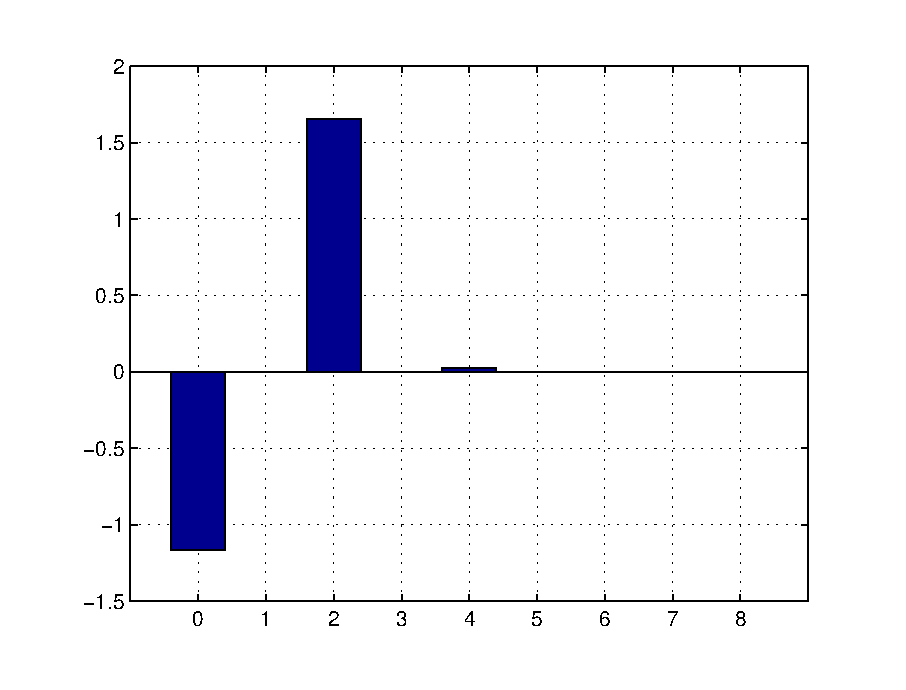
\includegraphics[scale=0.7]{\dirslike/vrsta_protokola_ys_1}
	\caption{AAmplitude harmonikov protokola}
	\label{fig:vrsta_protokola_ys_1}
\end{figure}


\subsection{Napaka pri dinami"cni ekscentri"cnosti v smeri x-osi}
\label{Napaka pri dinami"cni ekscentri"cnosti v smeri x-osi}

"Ze iz analiti"cnih izrazov lahko pri"cakujemo, da bo tu manj"sa izrazitost drugega harmonika. Napaka kota $\varepsilon$ je prikazana na sliki \ref{fig:protokol_xd_1}. Izrazit je predvsem prvi harmonik. Nezanemarljiv je "se drugi harmonik, ostale komponente Fourierjeve vrste pa so zanemarljive.

  \begin{figure}[h!]
  	\begin{center}
  		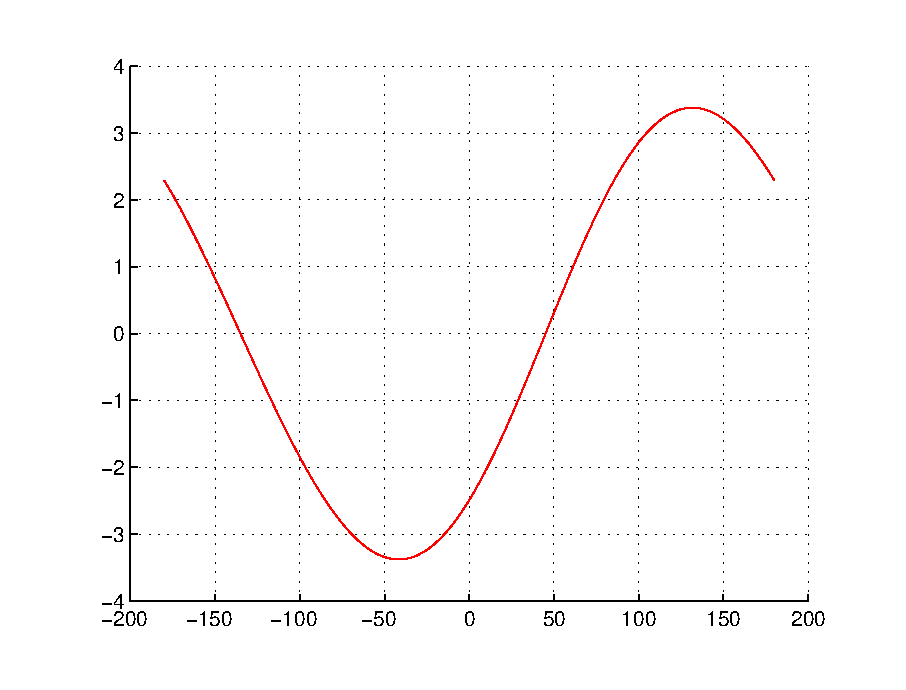
\includegraphics[scale=0.5]{\dirslike/protokol_xd_1.eps} %vrednost_polja_real.m
  	\end{center}
  	\caption{numericen izracun napake}
  	\label{fig:protokol_xd_1}
  \end{figure}
\begin{figure}
	
	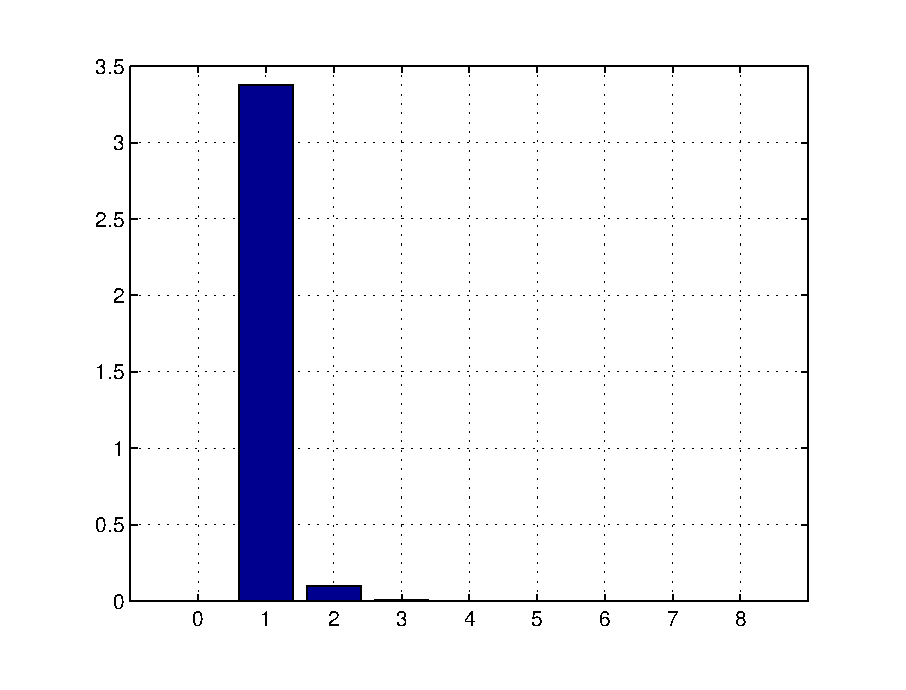
\includegraphics[scale=0.7]{\dirslike/vrsta_protokola_xd_1}%vrednost_polja_real.m
	\caption{AAmplitude harmonikov protokola}
	\label{fig:vrsta_protokola_xd_1}
\end{figure}






\section{Linearno ve"canje napake in opazovanje posameznih harmonikov pogre"ska}


Sedaj poglejmo kako se spreminja posamezna amplituda ekcentri"cnosti glede na velikost ekscentri"costi. Posami"cno sem ve"cal ekscentri"cnosti in pri tem opazoval spreminjanje pogre"ska $\varepsilon$. Pogre"sek $\varepsilon$ sem razvil v fourierovo vrsto in opazoval amplitudo posameznega harmonika $A_n \cos( n \theta)+B_n \sin(n \theta)$.


\subsection{Ve"canje stati"cne napake v x-osi}
Z ve"canjem stati"cne napake se spreminja amplituda posameznih harmonikov. Slika \ref{fig:potek_amplitude_harmonikov_xs} prikazuje potek amplitud posameznih harmonikov poteka napake $\varepsilon$. Opazimo dokaj linearno pove"cevanje amplitude posameznega harmonika. Vednost amplitude lahko zapi"semo kot polinom druge stopnje.
\begin{equation}
\label{eq:polinom_A0_xs}
A_0(\Delta x_s)=0.24856 \Delta x_s^3-2.334952 \Delta x_s^2+11.8579362 \Delta x_s +0.00749
\end{equation}
\begin{equation}
\label{eq:polinom_A2_xs}
A_2(\Delta x_s)=0.61989 \Delta x_s^3-4.32207 \Delta x_s^2+11.62794 \Delta x_s +0.02824
\end{equation}
\begin{equation}
\label{eq:polinom_B2_xs}
B_2(\Delta x_s)=0.32657 \Delta x_s^3+0.45499 \Delta x_s^2-12.04424 \Delta x_s +0.00516
\end{equation}

S primerjavo z analiti"cnih izpeljav lahko vidimo, da se pri majhnih ekscentri"cnostih amplitude harmonikov pogre"ska $\varepsilon$ linearno pove"cujejo.

%Vrednost enosmerne komponente lahko zapisemo kot polinom  v odvisnsti od $p_0(\Delta x_s)$. 

\begin{figure}[h!]
	
	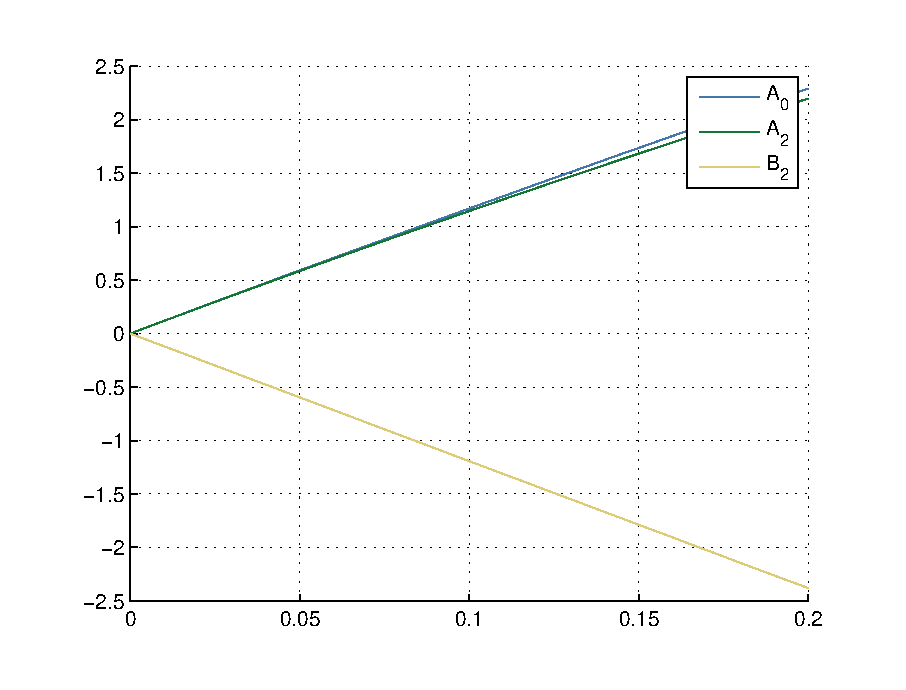
\includegraphics{\dirslike/potek_amplitude_harmonikov_xs} %uporaba_funkcije_vrednost_polja.m in nato Izris_potekov_amplitud.m
	\caption{AAmplitude harmonikov s spreminjanjem ekscentri"cnosti}
	\label{fig:potek_amplitude_harmonikov_xs}
\end{figure}

\subsection{Ve"canje stati"cne ekscentri"cnosti v y-osi}

Na sliki \ref{fig:potek_amplitude_harmonikov_ys} vidimo spreminjanje amplitude izrazitih posameznih harmonikov. Pri stati"cni ekscentri"cnosti v smeri y-osi se velikosti amplitud pri dolo"ceni ekscentri"cnosti ne spremeni. Spremeni se le predznak. Predznak sa spremenila amplituda enosmerne komponente in sinusna komponenta. S zapisom odvistnosti amlitude od ekscentri"cnosti s polinomom dobimo izraze:




\begin{equation}
\label{eq:polinom_A0_ys}
A_0(\Delta y_s)=-0.24299 \Delta y_s^3+2.33829 \Delta y_s^2-11.87186 \Delta y_s -0.00587
\end{equation}
\begin{equation}
\label{eq:polinom_A2_ys}
A_2(\Delta y_s)=0.85111 \Delta y_s^3-4.800845 \Delta y_s^2+11.88757 \Delta y_s +0.00263
\end{equation}
\begin{equation}
\label{eq:polinom_B2_ys}
B_2(\Delta y_s)=-0.33333 \Delta y_s^3-0.45861 \Delta y_s^2+12.0461 \Delta y_s -0.00527
\end{equation}
Izrazi (\ref{eq:polinom_A0_ys}),(\ref{eq:polinom_A2_ys}) in (\ref{eq:polinom_B2_ys}) so podobni izrazom (\ref{eq:polinom_A0_xs}),(\ref{eq:polinom_A2_xs}) in (\ref{eq:polinom_B2_xs}). Razlikujejo se le v predznakih pri izrazih (\ref{eq:polinom_A0_xs}) in (\ref{eq:polinom_B2_xs}). Razlika pri decimalnih mesti se pojavi zaradi numeri"cnih napak in kon"cnega "stevila to"ck s  katerimi sem aproksimiral polinom.



\begin{figure}[h!]
	
	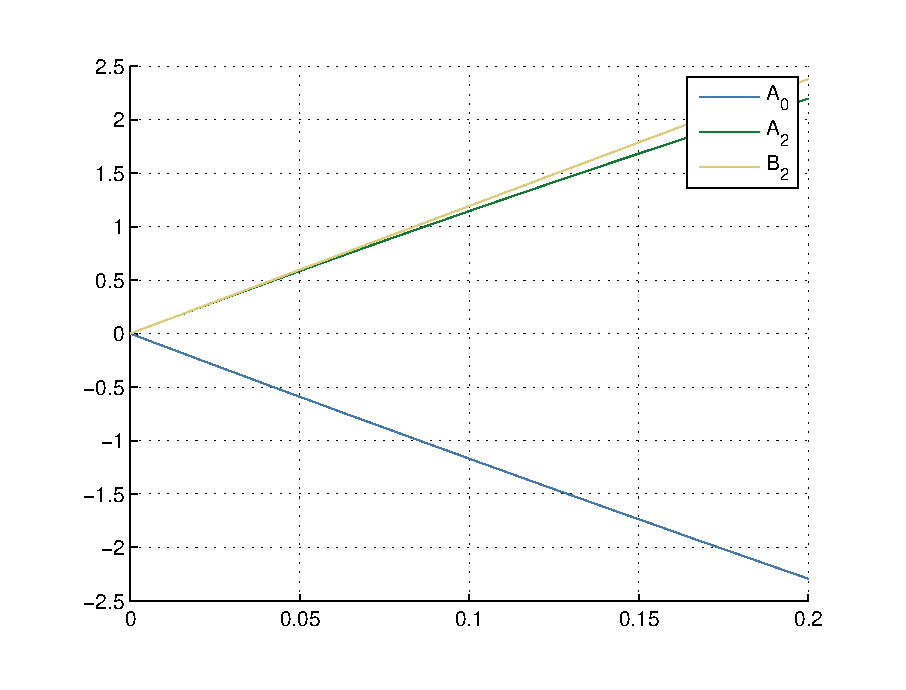
\includegraphics{\dirslike/potek_amplitude_harmonikov_ys}%uporaba_funkcije_vrednost_polja.m in Izris_potekov_amplitud.m
	\caption{AAmplitude harmonikov s spreminjanjem ekscentri"cnosti}
	\label{fig:potek_amplitude_harmonikov_ys}
\end{figure}


\subsection{Ve"canje dinami"cne napake v x-osi}

"Ze v poglavju \ref{Napaka pri dinami"cni ekscentri"cnosti v smeri x-osi}, smo opazili, da se pri dinami"cni ekscentri"cnosti napaka $\varepsilon$ pojavi v izraziti obliki prvega harmonika. Na sliki \ref{fig:potek_amplitude_harmonikov_xd} vidim potek amplitude prvega in drugega harmonika.  Z aproksimacijo, posamezne amplitude od dinami"cne ekscentri"cnosti v smeri x-osi, s polinomom dobimo izraze:

\begin{equation}
\label{eq:polinom_A1_xd}
A_1(\Delta x_d)=-0.6196 \Delta x_d^3+0.71962 \Delta x_d^2-24.09233 \Delta x_d+0.01225
\end{equation}
\begin{equation}
\label{eq:polinom_B1_xd}
B_1(\Delta x_d)=0.52925 \Delta x_d^3-0.50255 \Delta x_d^2+24.00878 \Delta x_d-0.00688
\end{equation}
\begin{equation}
\label{eq:polinom_A2_xd}
A_2(\Delta x_d)=0.17300\Delta x_d^3-9.97085\Delta x_d^2-0.02442\Delta x_d+0.00272
\end{equation}
\begin{equation}
\label{eq:polinom_B2_xd}
B_2(\Delta x_d)=-1.64858 \Delta x_d^3+1.6394\Delta x_d^2-0.45992\Delta x_d+0.02430
\end{equation}

Iz izrazov vidimo linearno nara"scanje amplitude prvega harmonika. Z ve"canjem eksentri"cnosti pri"cne kvadrati"cno nara"s"cati tudi drugi harmonik.


\begin{figure}[h!]
	
	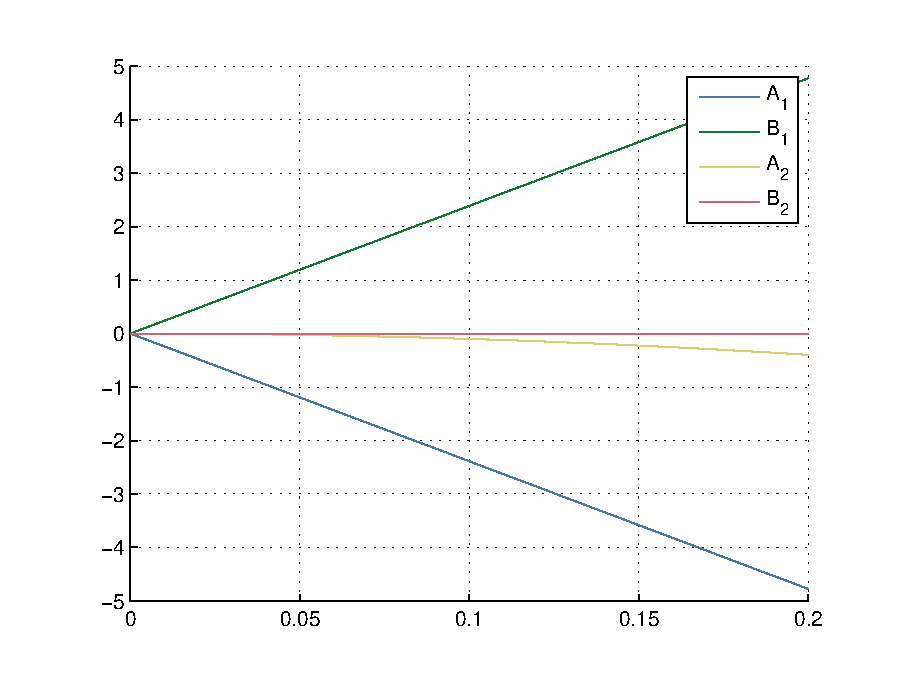
\includegraphics{\dirslike/potek_amplitude_harmonikov_xd} %uporaba_funkcije_vrednost_polja.m in nato Izris_potekov_amplitud.m
	\caption{AAmplitude harmonikov s spreminjanjem ekscentri"cnosti}
	\label{fig:potek_amplitude_harmonikov_xd}
\end{figure}


\section{Izra"cun napke z realnimi podatki gostote magnetnega polja}

V podjetju RLS merilna tehnika so mi simulirali Z-komponento vektorja gostote magnetnega pretoka. Simulacija je bila opravljena na vi"sini 2.55mm nad magnetom tako kot to predpisuje podotkovni list senzorja RM44. Kljub realnemu polju se zavedam da bo to"cnost simulacije slab"sa od realnega senzorja, saj merim polje le z dvema sondama. Sondi sem postavil na enak radij, kot so postavljene sonde v senzorju. S spreminjanjem radija na katerega sem postavil sondi se je spreminjala tudi velikost napake. Napaka je bila glede na dimenzije magneta najni"zja pri postavitvi sond na radij 2.4mm.  Simulacije sem se lotil na enak na"cin kot pri predpostavki, da je gostota magnetnega polja linearna funkcija. 




S poznavanjem lokacije sonde, sem iz tabele rezultatov simulacije Z-komponente vektorja B, od"cital polje. 

Izra"cun vrednosti polja v dolo"ceni to"cki z uporabo funkcije interp2 je dolgotrajen. Funkcija interp2 ima velik povpre"cni "cas izvajanja (ACET-avrage case execution time). Za hitrej"se izvajanje simulacije, sem zato za vrednost polja v dolo"ceni to"cki uporabil vrednost polja, v kateri imam znano polje in je le ta najbli"zja to"cki v kateri "zelim dobiti polje. Simulacije sem opravil tudi z uporabo funkcije interp2. () Razlika dobljenih potekov vektorja B je vidna na sliki (dodaj sliko !!!!!!). Razlika ni velika, "cas izvajanja simulacije pa je kraj"si. 

Tako sem dobil poteke vektorja B, ki ga pomeriti sondi v odvistnosti od trenutnaga zasuka $\theta$. Nato sem z uporabe funkcije atan2 dolo"cil vrednost kota $\varphi$. 



Podatek, ki me je zanimal, je seveda napaka. V naslednjih podpoglavjih bom predstavil, potek napake $\varepsilon$ v odvistnosti od kota zasuka $\theta$, z uporabo realnega vektorja B ki ga ustvarja magnet.

 


\subsection{Napaka brez ekscentri"cnosti}

Poglejmo najprej kak"sen je potek napake brez ekscentri"cnosti. Potek napake $\varepsilon$ se nahaja na sliki \ref{fig:protokol_real_brez}. Opazimo da je nekoliko bolj izrazit "cetrti harmonik, ki pri simulacijah ekscentri"cnosti z aprksimacijo linearnega vektorja B ni bil klju"cen. Ve"cji skoki ki se pojavljajo v napaki (kot naprimer pri $\theta=-160^\circ$), so posledica numeri"cne napake pri simulaciji Z komponente vektorja B. 


\begin{figure}[h!]
	
	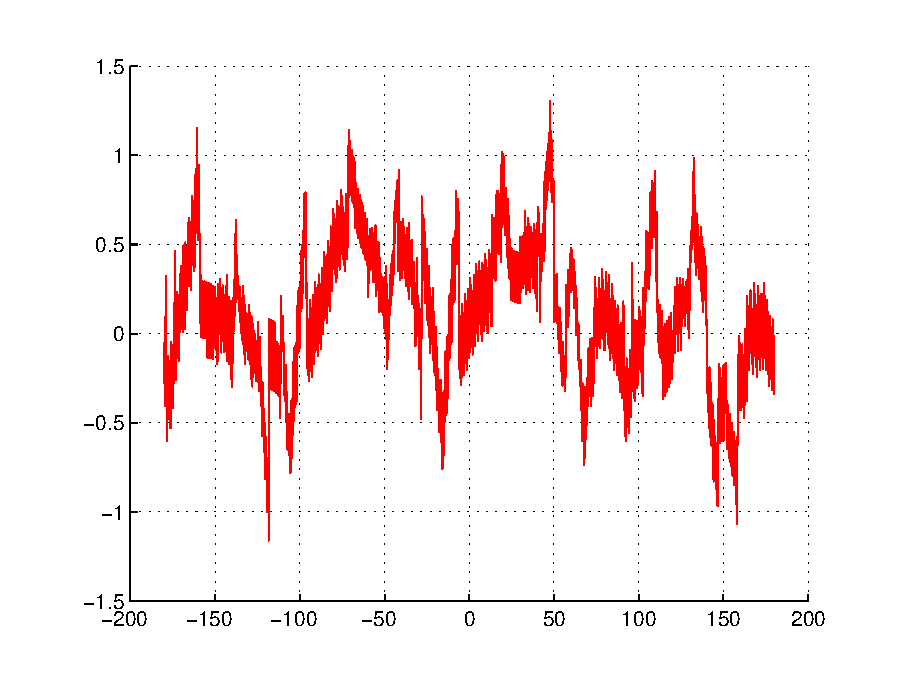
\includegraphics[scale=0.5]{\dirslike/protokol_real_brez}%vrednost_polja_real.m
	\centering
	\caption{Napaka pomerjenega kota pri idealni montazi}
	\label{fig:protokol_real_brez}
\end{figure}

Z razvojem napake $\varepsilon$ v Fouriejevo vrsto, se potrdi teza da je najvi"sji "cetrti harmonik. Pri uporabi linearnega polja vektorja B se je stati"cno ekscentri"cnostjo najbolj spreminjala amplituda drugega harmonika, katera je v napaki na sliki \ref{fig:amplitude_real_brez} majhna. Vi"sje harmonike bi lahko izlo"cil "ce bi uporabil ve"c Hallovih sond. Sonde bi morale biti pametno razporejene po radiju, tako kot je to vrjetno izvedeno v senzorju RM44.

\begin{figure}[h!]
	
	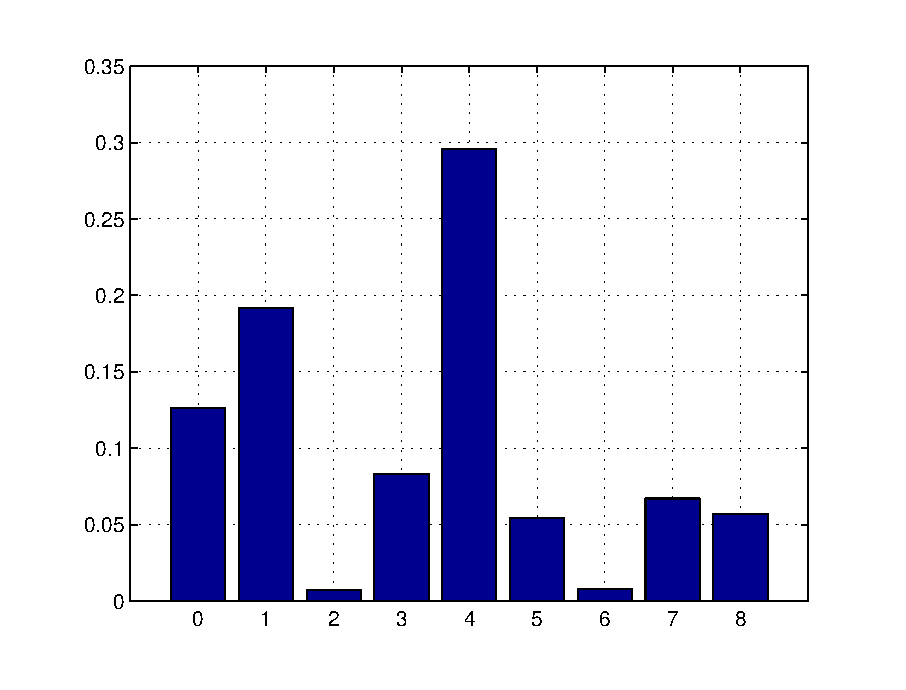
\includegraphics[scale=0.5]{\dirslike/vrsta_protokola_real_brez}%vrednost_polja_real.m
	\centering
	\caption{Amplitude harmonikov pogre"ska $\varepsilon$}
	\label{fig:amplitude_real_brez}
\end{figure}

\subsection{Napaka pri stati"cni ekscentri"cnosti v smeri x-osi}


Sedaj v simulaciji dodamo stati"cno ekscentri"cnost v smeri x-osi. Razlika med izra"cunanim kotom $\varphi$ in pravim kotom $\theta$,v odvistnosti od pravilnega kota $\theta$ je prikazana na sliki \ref{fig:protokol_real_xs}. Tako kot je v napaki pri uporabi linearnega vektorja B najbolj izstopala enosmerna komponenta in drugi harmonik, se tudi tu takoj opazi podoben potek.

\begin{figure}[h!]
	
	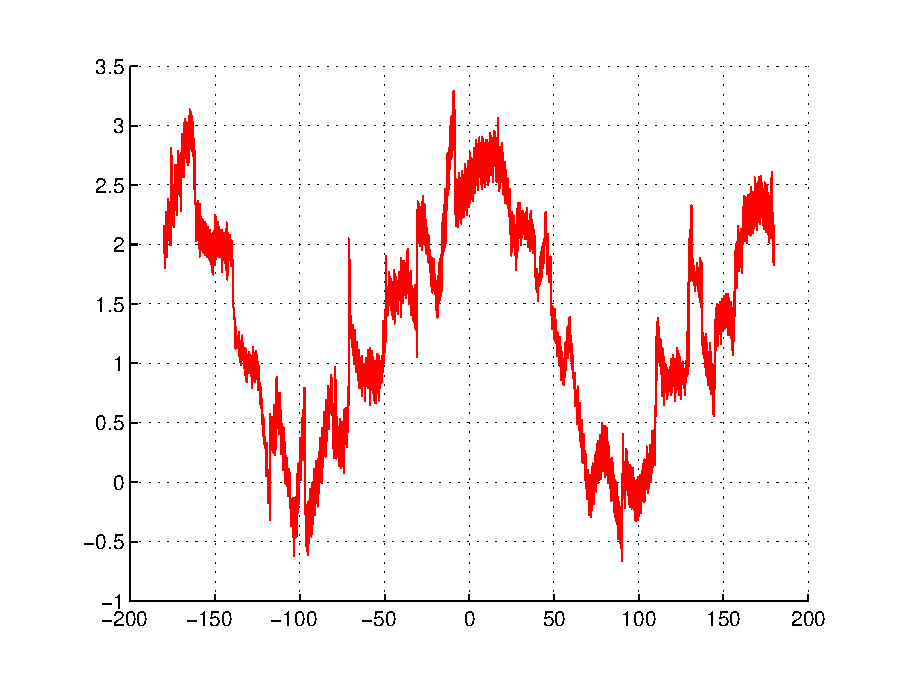
\includegraphics[scale=0.5]{\dirslike/protokol_real_xs_1}%vrednost_polja_real.m
	\centering
	\caption{Napaka pomerjenega kota pri stati�cni ekscentri�nosti v smeri x-osi }
	\label{fig:protokol_real_xs}
\end{figure}

Z razvojem napake v Fourijejevo vrsto (slika \ref{fig:amplitude_real_xs}) lahko vidimo podobnosti, z napako, kjer je bilo uporabljeno linearno polje vektorja B. Izstopati enosmerna komponta in drugi harmonik. Malo izstopa tudi "cetrti harmonik, ostali so zanemarljvi.


\begin{figure}[h!]
	
	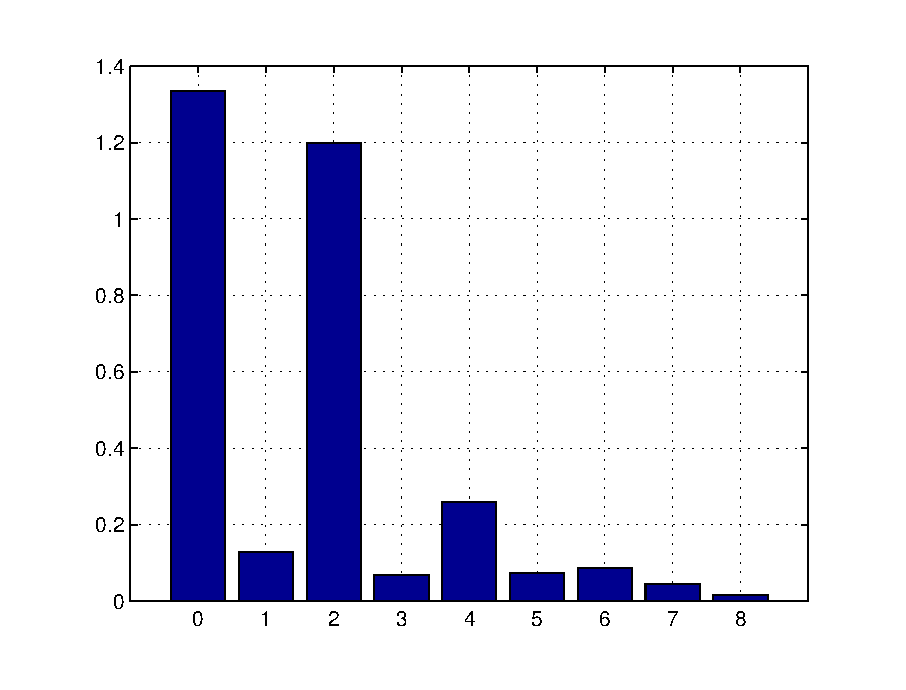
\includegraphics[scale=0.5]{\dirslike/vrsta_protokola_real_xs_1}%vrednost_polja_real.m
	\centering
	\caption{Amplitude harmonikov pogre"ska $\varepsilon$ ob stati"cni ekscentri"cnosti v smeri x-osi}
	\label{fig:amplitude_real_xs}
\end{figure}



\subsection{Napaka pri stati"cni ekscentri"cnosti v smeri y-osi}

Po simulacijah z uporabo linearnega polja sem pri"cakoval enak potek napake kot pri stati"cni ekscentri"cnosti v smeri x-osi. Pri"cakoval sem razliko le v enosmerni komponenti, ki bo negativna, drugi harmonik pa fazno premaknjen.

Napaka $\varepsilon$ za primer ekscentri"cnosti v smeri y-osi, je prikazana na sliki \ref{fig:protokol_real_ys}. S slike se opazi pri"cakovano negativno enosmerno komponento in izrazit drugi harmonik. Razvoj napake $\varepsilon$ v Fourierovo vrsto potrdi pri"cakovane rezultate(slika \ref{fig:amplitude_real_ys}).

\begin{figure}[h!]
	
	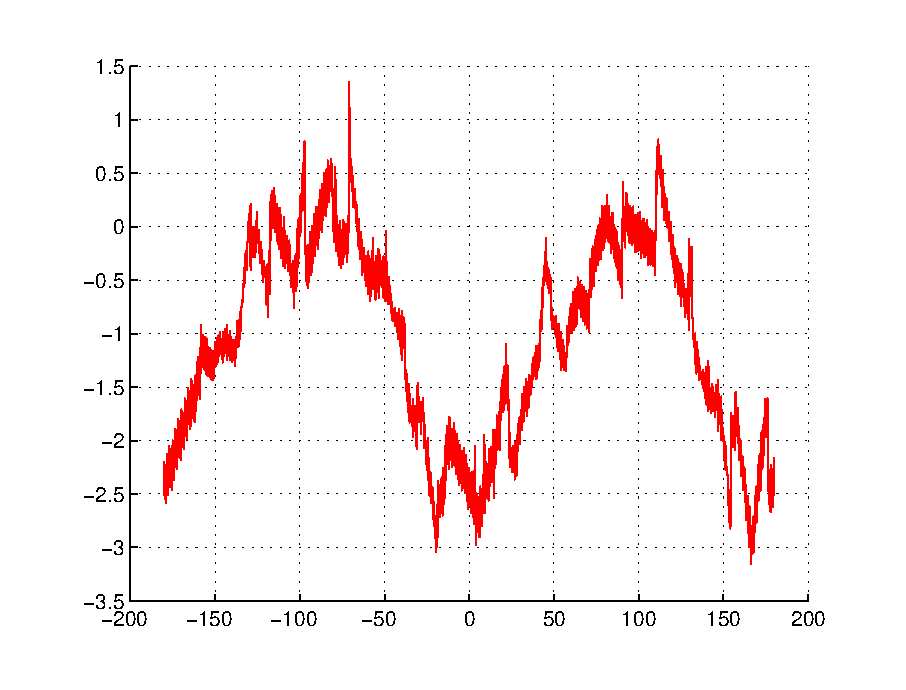
\includegraphics[scale=0.5]{\dirslike/protokol_real_ys_1}%vrednost_polja_real.m
	\centering
	\caption{Napaka pomerjenega kota pri stati�ni ekscentri�nosti v smeri y-osi }
	\label{fig:protokol_real_ys}
	\
\end{figure}


\begin{figure}[h!]
	
	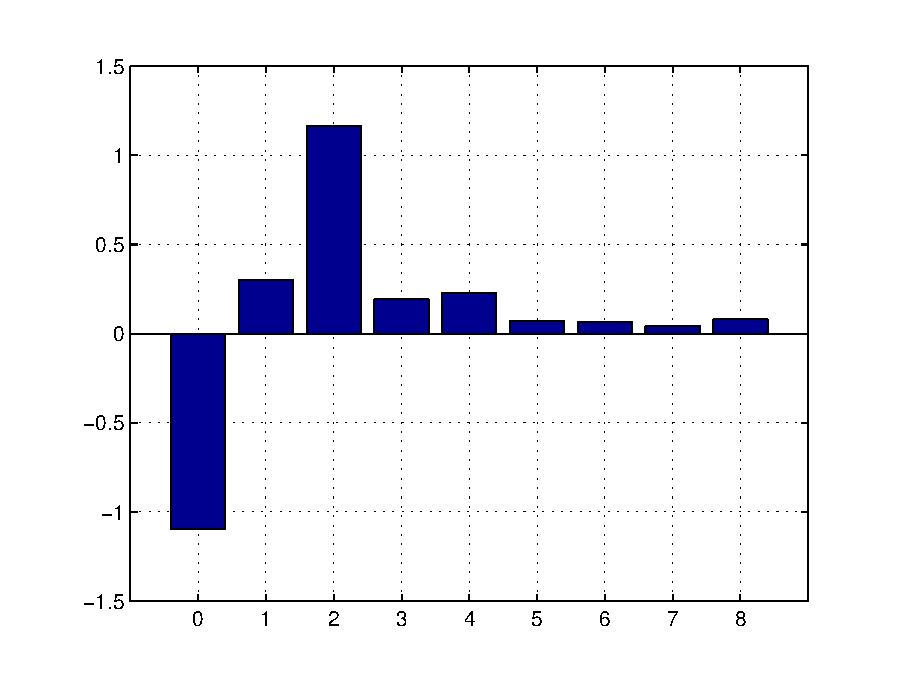
\includegraphics[scale=0.5]{\dirslike/vrsta_protokola_real_ys_1}%vrednost_polja_real.m
	\centering
	\caption{Amplitude harmonikov pogre"ska $\varepsilon$ ob stati"cni ekscentri"cnosti v smeri y-osi}
	\label{fig:amplitude_real_ys}
\end{figure}

\subsection{Napaka pri dinami"cni ekscentri"cnosti v smeri x-osi}

Pri dinami"cne ekscentir"cnosti sem pri"cakoval izrazit prvi harmonik napake. Napaka $\varepsilon$ prikazana na sliki \ref{fig:protokol_real_xd}. Na sliki opazimo izrazit tretji harmonik, ki je bil v napaki z uporabo linearnega polja B zanemarljiv. Z razvojem napake v Fourierovo vrsto (slika \ref{fig:amplitude_real_xd}) opazimo, da je amplituda tretjega harmonika podobna amplitudi prvega harmonika. Enosmerna komponenta je nizka po pri"cakovanjih. Ostali harmoniki imajo enake vrednosti kot napaka, kjer sem postavil ekscentri"cnosti na ni"c. Amplituda prvega harmonika je ni"zja od pri"cakovane vrednosti.
\begin{figure}[h!]
	
	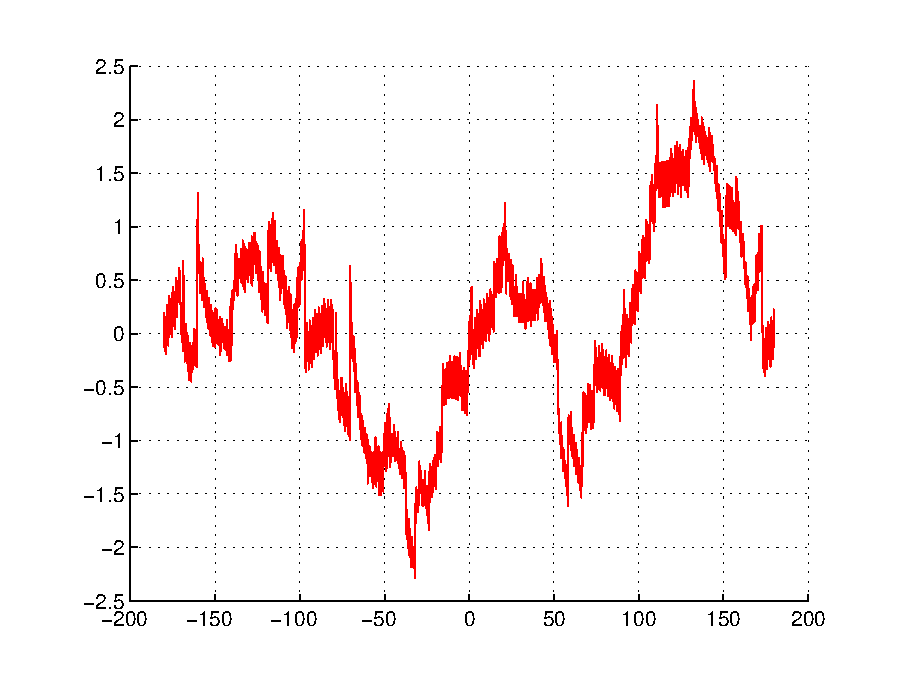
\includegraphics[scale=0.5]{\dirslike/protokol_real_xd_1}%vrednost_polja_real.m
	\centering
	\caption{Napaka pomerjenega kota pri dinami"cni ekscentri�nosti v smeri x-osi }
	\label{fig:protokol_real_xd}
\end{figure}

\begin{figure}[h!]
	
	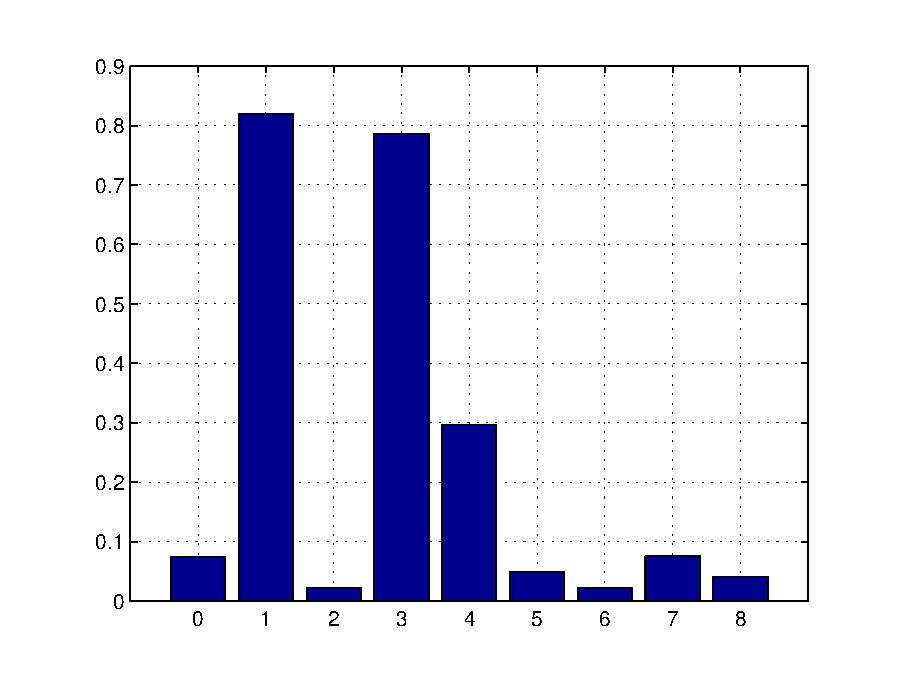
\includegraphics[scale=0.5]{\dirslike/vrsta_protokola_real_xd_1}%vrednost_polja_real.m
	\centering
	\caption{Amplitude harmonikov pogre"ska $\varepsilon$ ob dinami"cni ekscentri"cnosti v smeri x-osi}
	\label{fig:amplitude_real_xd}
\end{figure}

\subsection{Napaka pri dinami"cni ekscentri"cnosti v smeri y-osi}

Dinami"cna ekscentri"cnost v smeri y-osi ni bilo zaradi poenostavitve z uporabo linearnega polja B. Z uporabo realnega modela polja pri"cakujem napako podobno. Napaka je prikazana na sliki \ref{fig:protokol_real_yd}. Napaka je zelo podobena napaki dinami"cne ekscentri"cnosti v smeri x-osi z uporabo linearnega magnetnega polja B. Izrazit je prvi harmonik, izstopa tudi tretji. Z razvojem v Fouriejevo vrsto, opazimo izrazit prvi harmonik. Povi"sala se je amplituda tretjega harmonika, ostali harmoniki pa imajo amplitude zanemarljive.


\begin{figure}[h!]
	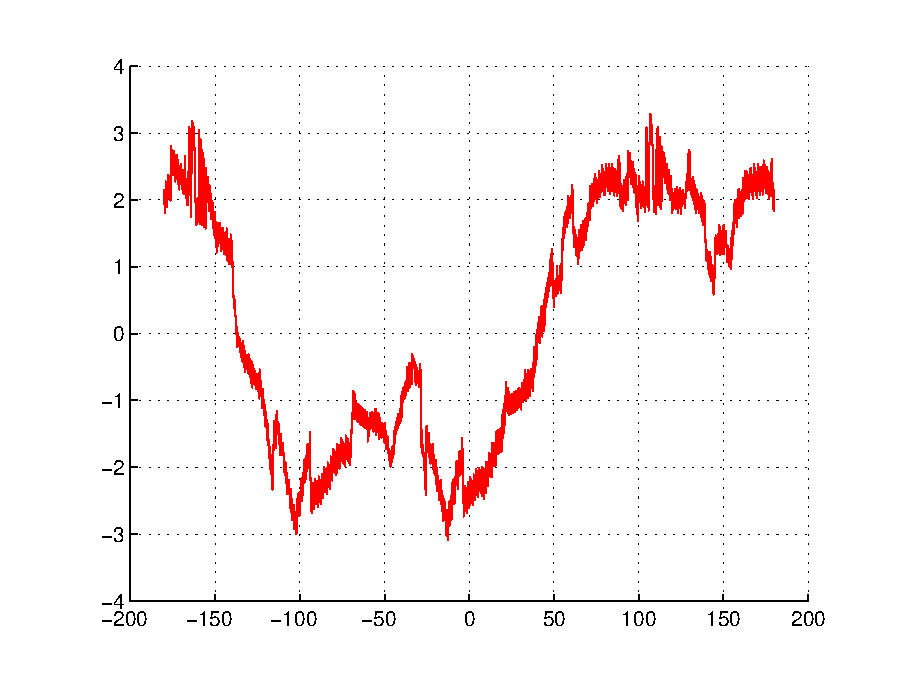
\includegraphics[scale=0.5]{\dirslike/protokol_real_yd_1}%vrednost_polja_real.m
	\centering
	\caption{Napaka pomerjenega kota pri dinami"cni ekscentri�nosti v smeri y-osi }
	\label{fig:protokol_real_yd}
\end{figure}

\begin{figure}[h!]
	
	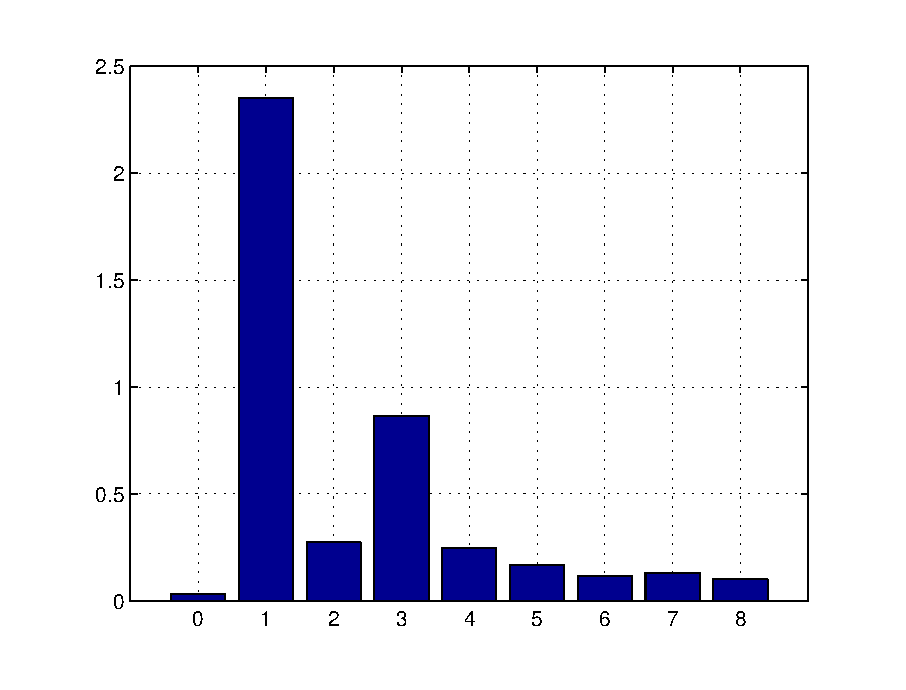
\includegraphics[scale=0.5]{\dirslike/vrsta_protokola_real_yd_1}%vrednost_polja_real.m
	\centering
	\caption{Amplitude harmonikov pogre"ska $\varepsilon$ ob dinami"cni ekscentri"cnosti v smeri y-osi}
	\label{fig:amplitude_real_yd}
\end{figure}





\subsection{Ve"canje stati"cne ekscentri"cnosti v x-osi}
\label{sec:vec_st_x}

Sedaj poglejmo odvistnost spreminjanja posamezne amplitude harmonikov v odvistnosti od stati"cne ekscentri"cnosti v smeri x-osi. Iz rezultatov kjer smo predpostavili linearno polje z-komponente vektorja B. Pri"cajkujem tudi tu podobne rezultate. Za"cetne vrednosti amplitud bodo neni"celne, saj "ze v primeru brez ekscentri"cnosti dobim napako, ki se izra"za v posameznih harmonikih(slika \ref{fig:amplitude_real_brez}).   Spremembo amplitude enosmerne komponente in drugega harmonika je vidna na sliki \ref{fig:potek_amplitude_harmonikov_xs_real}.





\begin{figure}[h!]
	
	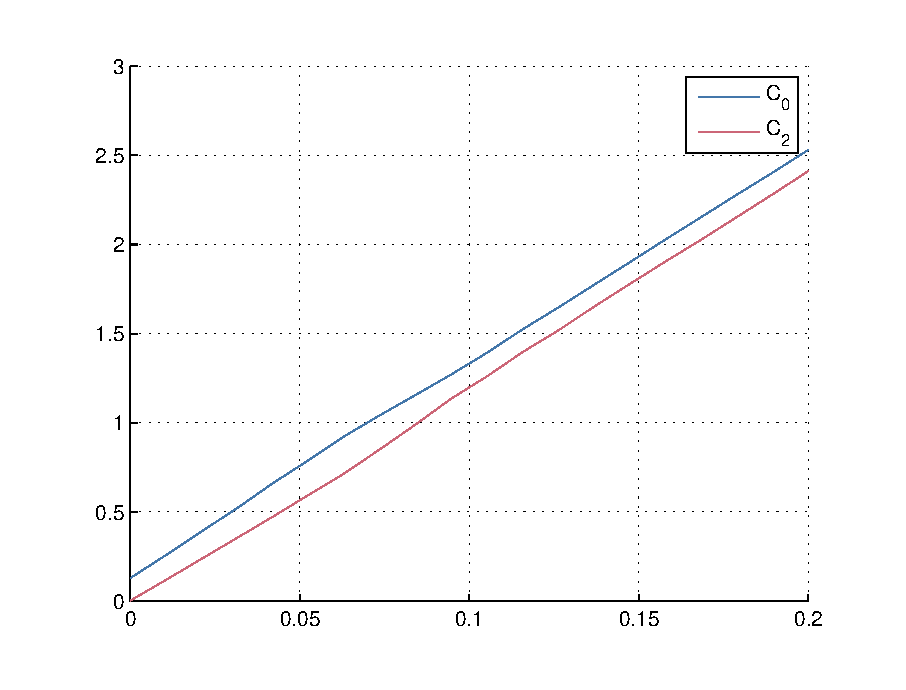
\includegraphics{\dirslike/potek_amplitude_harmonikov_xs_real} %uporaba_funkcije_vrednost_polja.m in nato Izris_potekov_amplitud.m
	\caption{Amplitude harmonikov s spreminjanjem ekscentri"cnosti}
	\label{fig:potek_amplitude_harmonikov_xs_real}
\end{figure}

Spreminjanje amplitude posameznega harmonika lahko aproksimiramo s polinomom tretje stopnje in dobimo izraz:

\begin{equation}
C_0(\Delta x_s)=39,78 \Delta x_s^3-13,29 \Delta x_s^2 +13,12 \Delta x_s+0,12
\end{equation}

\begin{equation}
C_2(\Delta x_s)=-61,68 \Delta x_s^3+19,77 \Delta x_s^2 +10,49 \Delta x_s+0,004
\end{equation}


Pri"cakovano je za"cetna vrednost aproksimacijskega polinoma enaka amplitudi harmonika pri napaki brez ekscentri"cnosti. Enosmerna kmponenta je nara"s"ca enako, kot je nara"s"cala pri simulaciji z uporabo linearnega polja z-komponente vektorja B, medtem ko amplituda drugega harmonika nara"s"ca po"casneje.


\subsection{Ve"canje stati"cne ekscentri"cnosti v y-osi}

Napaka zaradi stati"cne ekscentri"cnosti v smeri y-osi pri"cakujem enako kot pri ekscentri"cnosti v smeri x-osi. Po rezultatih iz prej"snjih poglavij predvidevam, da bo enosmerna komponenta z vi"sanjem ekscentri"cnosti vedno bolj negativna.

Na sliki \ref{fig:potek_amplitude_harmonikov_ys_real} so predvidevanja potrdijo. Za"cetni vrednosti sta enaki. Amplituda drugega harmonika nara"sca enako kot nara"sca amplituda drugega harmonika pri stati"cni ekscentri"cnosti v smeri x-osi. Odvistnost amplitude posameznega harmonika napake lahko aproksimiramo s polinomom. Potek je amplitude je po pri"cakovanjih.


\begin{figure}[h!]
	
	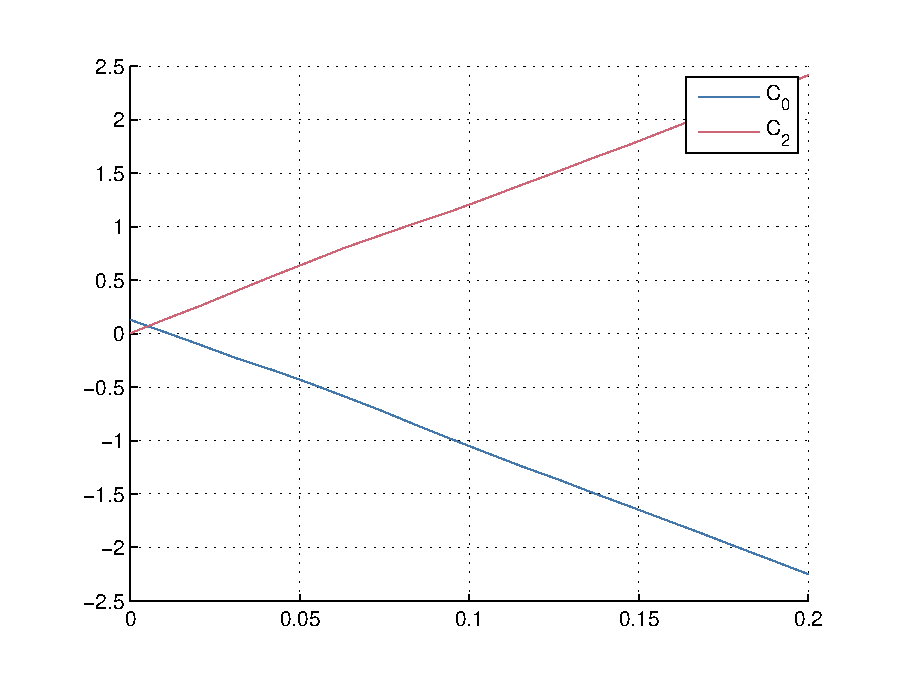
\includegraphics{\dirslike/potek_amplitude_harmonikov_ys_real} %uporaba_funkcije_vrednost_polja.m in nato Izris_potekov_amplitud.m
	\caption{Amplitude harmonikov s spreminjanjem ekscentri"cnosti}
	\label{fig:potek_amplitude_harmonikov_ys_real}
\end{figure}


\begin{equation}
A_0(\Delta y_s)=   
38.7884\Delta y_s^3
-13.0988\Delta y_s^2
-10.7638\Delta y_s
+0.1253
\end{equation}


\begin{equation}
C_2(\Delta y_s)= 
61.0142 \Delta y_s^3
-18.9682\Delta y_s^2+
13.4816\Delta y_s
-0.0028
\end{equation}




\subsection{Ve"canje dinami"cne ekscentri"cnosti v x-osi}
Pri simulacijah napake zaradi dinami"cne ekscentir"cnosti pri uporabi linearnega poteka z-komponente vektorja B je amplituda prvega harmonika linearno nara"scala v odvistnosti od ve"canja dinami"cne ekscentri"cnosti v smeri x-osi. Pri"cakujem linearno nara"s"cananje amplitude prvega harmonika. Pri simulaciji z realnim poljem se je izkazal za izrazitej"si tretji harmonik. Pri"cakujem, da bo tudi amplituda tretjega harmonika nara"s"cala z ve"canjem ekscentri"cnosti. Na sliki \ref{fig:potek_amplitude_harmonikov_xd_real} so prikazani poteki amplitud za prvi drugi in tretji harmonik v odvistnosti od dinami"cne ekscetri"cnosti v x-osi. Amplitudi prvega in tretjega harmonika nara"s"cata linearno in strmo. Drugi harmonik nara"s"ca s kvadratom ekscentri"cnosti vendar zelo polo"zno. Poteke amplitude posameznega harmonika v odvistnosti od dinami"cne ekscentri"cnosti v smeri x-osi lahko aproksimiramo s polinomom:
\begin{equation}
C_1(\Delta x_d)=   
-5.88\Delta x_d^3
+5.50\Delta x_d^2
+7.18\Delta x_d
+0.08
\end{equation}
\begin{equation}
C_2(\Delta x_d)=   
-0.31\Delta x_d^3
+0.95\Delta x_d^2
-0.09\Delta x_d
+0.004
\end{equation}
\begin{equation}
C_3(\Delta x_d)=   
-3.28\Delta x_d^3
+2.52\Delta x_d^2
+8.19\Delta x_d
-0.04
\end{equation}


\begin{figure}[h!]
	
	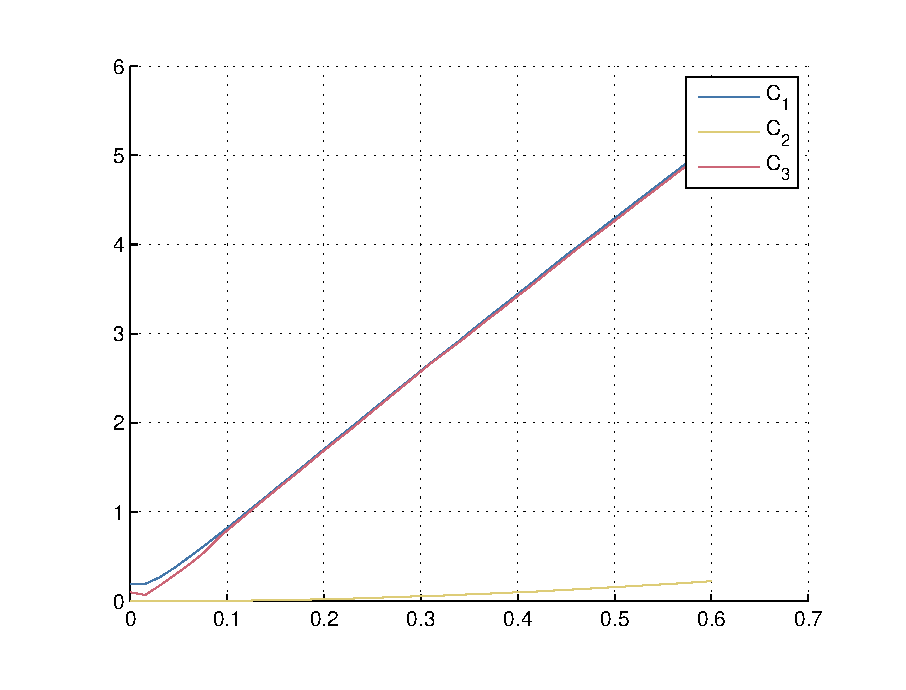
\includegraphics{\dirslike/potek_amplitude_harmonikov_xd_real} %uporaba_funkcije_vrednost_polja.m in nato Izris_potekov_amplitud.m
	\caption{Amplitude harmonikov s spreminjanjem ekscentri"cnosti}
	\label{fig:potek_amplitude_harmonikov_xd_real}
\end{figure}


\subsection{Ve"canje dinami"cne ekscentri"cnosti v y-osi}

Pri dinami"cni ekscentri"cnosti v smeri y-osi pri"cakujem podobne rezultate kot pri dinami"cni ekscentri"cnosti v smeri x-osi. Pri"cakujem le vi"sjo amplitudo prvega harmonika. Rezultat je viden na sliki \ref{fig:potek_amplitude_harmonikov_yd_real}. Amplituda prvega harmonika nara"s"ca pribli"zno trikrat hitreje, kot je nara"s"cala amplituda prvega haromika pri dinami"cni ekscentri"cnosti v smei x-osi. Drugi harmonik nara"s"ca po"casneje kot pri dinami"cni ekscentri"cnosti v smei x-osi, tretji harmonik poteka pribli"zno enako.
Aproksimacija s polinomom potrdi sklepanja s slike.


\begin{figure}[h!]
	
	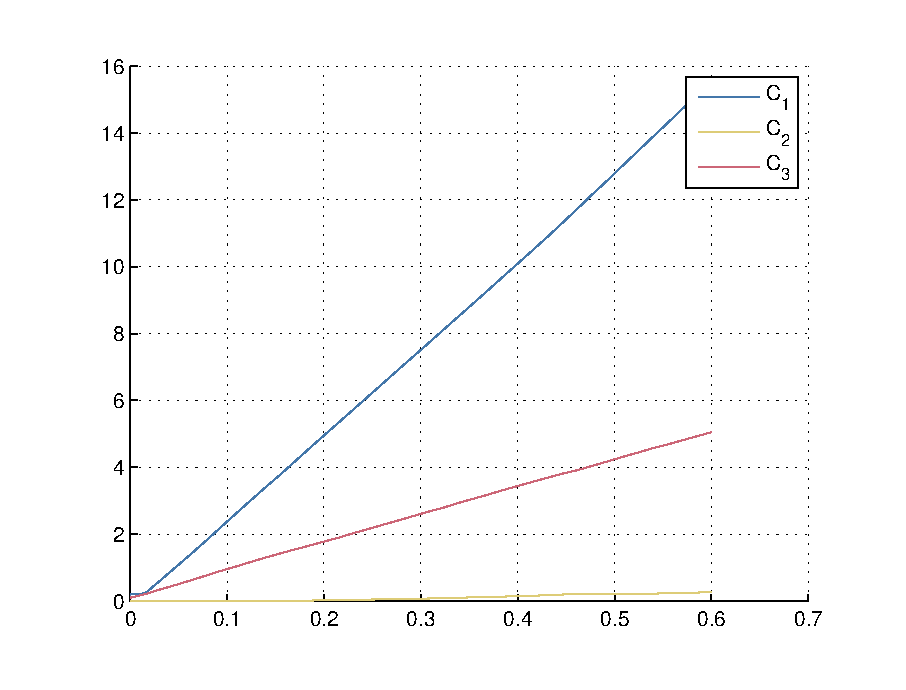
\includegraphics{\dirslike/potek_amplitude_harmonikov_yd_real} %uporaba_funkcije_vrednost_polja.m in nato Izris_potekov_amplitud.m
	\caption{Amplitude harmonikov s spreminjanjem ekscentri"cnosti}
	\label{fig:potek_amplitude_harmonikov_yd_real}
\end{figure}
\begin{equation}
C_1(\Delta y_d)=   
1.01\Delta y_d^3
+1.82\Delta y_d^2
+24.57\Delta y_d
-0.07
\end{equation}
\begin{equation}
C_2(\Delta y_d)=   
-2.37\Delta y_d^3
+2.79\Delta y_d^2
-0.41\Delta y_d
+0.01
\end{equation}
\begin{equation}
C_3(\Delta y_d)=   
0.83\Delta y_d^3
-1.21\Delta y_d^2
+8.71\Delta y_d
+0.09
\end{equation}

\section{Zaklju"cna misel po opravljenih simulacijah}
Predvidevam, da bo pri meritvah napaka ni"zja, saj je bil simulacijski model osnoven. V napaki kljub temu pri"cakujem izraz napake v obliki enosmerne komponente oz. prvega ali drugega harmonika. Napaka bo z ve"canjem ekscentri"cnosti nara"s"cala pribli"zno linearno. Napaka zaradi dinami"cne ekscentri"cnosti bo vi"sja kot napaka zaradi stati"cne ekscentri"cnosti. To se je pokazalo "ze pri linearnem modelu in prav tako prirealnem modelu polja.



\chapter{Meritve ekscentri"cnosti}

Meritve ekscentri"cnosti sem opravil na napravi v LRTME. Naprava omogo"ca premik senzorja v "sestih prostorskih smereh. Potreboval sem le dve. Za referen"cni enkoder je uporabljen encoder Tonic T2001-15A podjetja Renishaw.

Senzor RM44 pomeri magnetno polje s ve"cjim "stevilom Hallovih senzorjev. Z matemati"cno obdelavo signalov s Hall-ovih sond prejmem na izhodu senzorja dva analogna signala.
Analogna  signala prikazujeta enako vrednost kot "ce bi pomeril magnetno polje magneta z dvema Hall-ovima sondama, ki sta prostorsko premaknjeni za $90^\circ$. 
Iz prejetih signalov s funkcijo $\arctan$ lahko izra"cunam trenutno pozicijo. Postopek je enak postopku, ki sem ga uporabil med simulacijam.


\section{Pomerjeno magnetno polje}

Na za"cetku si oglejmo prejeta signala s senzorja. V idelani monta"zi oz. vkolikor sem senzor lahko 


\subsection{Napaka ko sta senzor in magnet na isti osi}

napaka med kotom pomerjenega s senzorjem RM44 in referen"cnim enkoderjem je prikazana na sliki \ref{fig:protokol_merjeni_brez}. 




\begin{figure}[h!]
	
	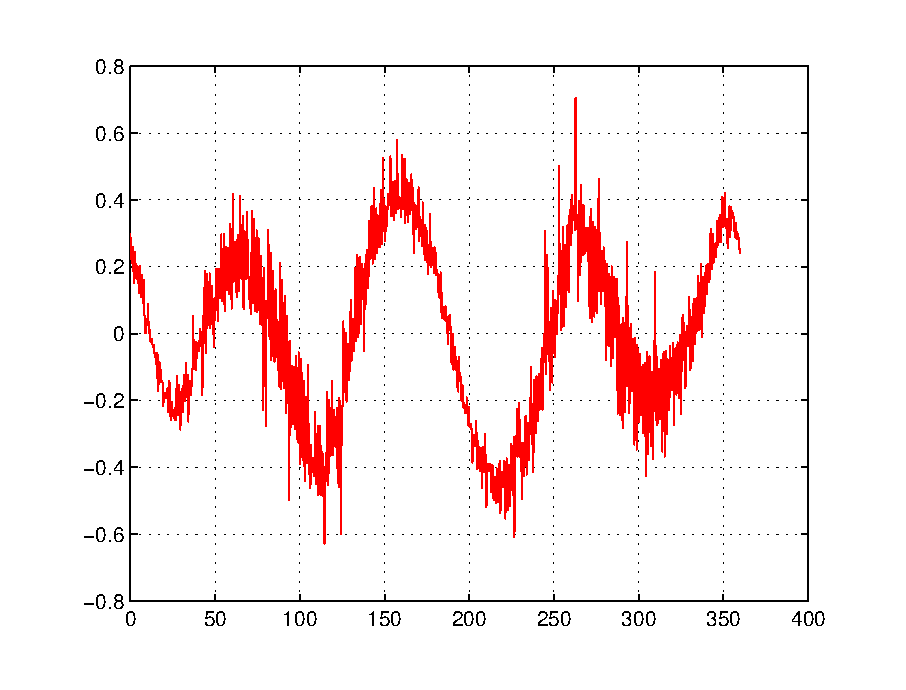
\includegraphics[scale=0.5]{\dirslike/protokol_meritve_brez.eps} % izpis_harmonikov.m
	\caption{Napaka pomerjenega kota pri najbolj"simonta"zi}
	\label{fig:protokol_merjeni_brez}
\end{figure}

V napaki je najizrazitej"si "cetrti harmonik. Vi"sja frekvenca vidna v napaki je razlika ki nastane zaradi razli"cnih resolucij enkoderjev. Izhoda senzorja (signala sinus in kosinus), sta z analogno-digitalnim pretvorniko pretvorjena v digitalno obliko. AD pretvornik ima ni"zjo resolucijo kot referen"cni enkoder.

S primerjavo napake pri simulacijah z realnim poljem, ko je bil senzor in magnet v idealne stanju (Slika \ref{fig:protokol_real_brez}) opazimo, da je napaka manj"sa. Napaka je manj"sa zaradi drugega na"cina zajema signalov sinus in kosinus.

Napako razvijmo v Fourierovo vrsto. Amplituda posameznega harmonika je prikazana na sliki \ref{fig:amplitude_merjeni_brez}. Enosmerna komponenta je ni"c, saj se ob zagonu naprave senzora kalibrirata v enako izhodi"sce. Nara"s"canje enosmerna komponenta se bo pojavila z izmikom senzorja iz kalibrirane pozicije. S primerjavo velikosti amplitud posameznega harmonika napake pri simulacijah z uporabo realnega magnetnega polja (slika \ref{fig:amplitude_real_brez}) opazimo, da je amplituda drugega harmonika vi"sja kot amplituda drugega harmonika pri simulacijah. 

\begin{figure}[h!]
	
	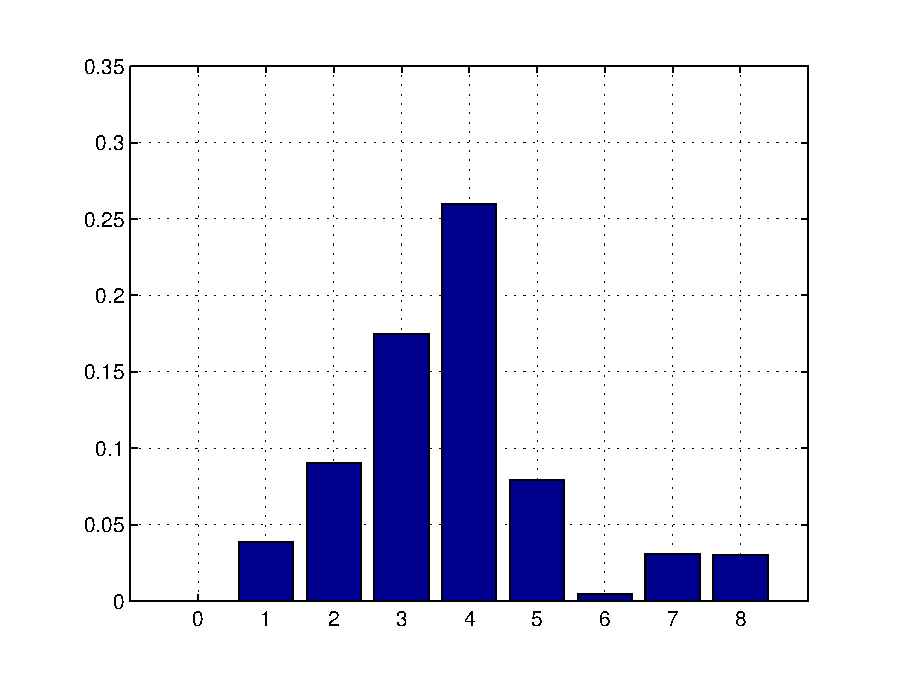
\includegraphics[scale=0.5]{\dirslike/vrsta_protokola_meritve_brez.eps} % izpis_harmonikov.m 
	\caption{Amplitude posameznega  harmonika napake pri najbolj"si monta"zi}
	\label{fig:amplitude_merjeni_brez}
\end{figure}


\subsection{Napaka pri stati"cni ekscentri"cnosti v smeri x-osi}

Pri simulcijah stati"cne ekscentri"cnosti se je pojavila napaka v obliki drugega harmonika. Napako pri meritvah pri"cakujem manj"so kot je bila v simulacijah. Pri"cakujem enako obliko. Napaka pri ekscentri"cnosti 0.1mm je prikazana na sliki \ref{fig:protokol_merjeni_xs_1}. Napaka je v primerjavi s simulacijami pol manj"sa (slika \ref{fig:amplitude_real_xs}). Iz poteka napake ni razvidno, povi"sanje le drugega harmonika. 

Slika  \ref{fig:amplitude_merjeni__xs_1} prikazuje amplitude posameznih harmonikov v napaki. Po pri"cakovanjih sta se povi"sali enosmerna komponenta in drugi harmonik. Po nepri"cakovanem se je povi"sal tudi prvi harmonik. Med simuliranjem nisem zaznal, da bi bile napake ekscentri"cnosti odvisne od drugih ekscentri"cnosti. Amplituda prvega harmonika napake je najvi"sja. Harmoniki, vi"sji od drugega se z ekscentri"cnostjo niso spremnili.



\begin{figure}[h!]
	
	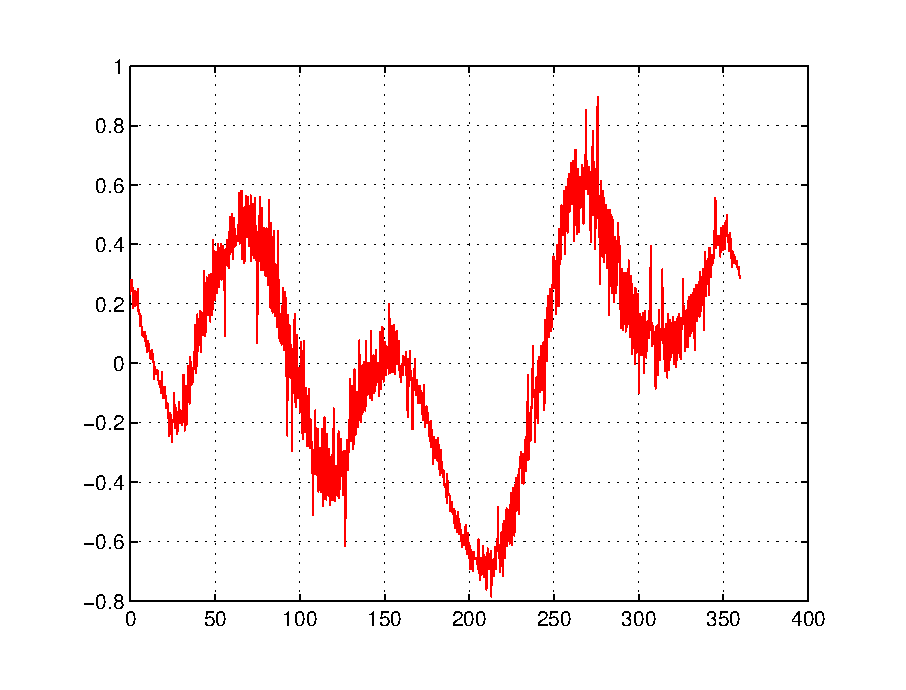
\includegraphics[scale=0.5]{\dirslike/protokol_meritve_xs_1.eps} % izpis_harmonikov.m
	\caption{Napaka pomerjenega kota pri stati"cni ekscentri"cnosti v x-osi}
	\label{fig:protokol_merjeni_xs_1}
\end{figure}




\begin{figure}[h!]
	
	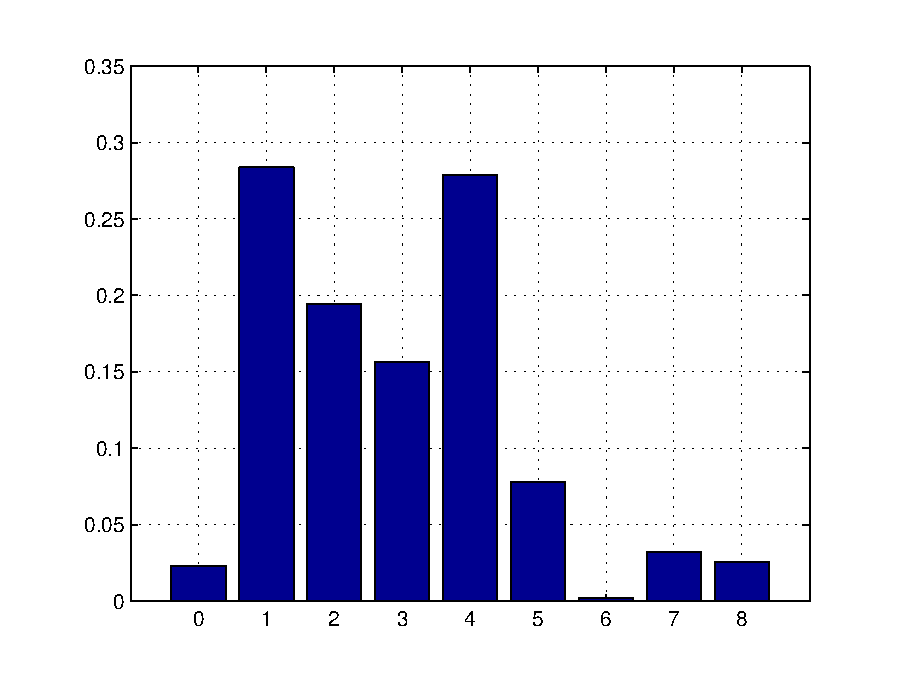
\includegraphics[scale=0.5]{\dirslike/vrsta_protokola_meritve_xs_1.eps} % izpis_harmonikov.m
	\caption{Razvoj napake v F vrsto pri stati"cni ekscentri"cnosti v x-osi}
	\label{fig:amplitude_merjeni__xs_1}
\end{figure}





\subsection{Napaka pri stati"cni ekscentri"cnosti v smeri y-osi}



Izmaknimo sedaj senzor v smeri y-osi. Opazi se pozitivno enosmerno komponento katero sem iz rezultatov simulacij pri"cakoval negativno (Slika \ref{fig:protokol_merjeni_ys_1}). Napaka je ve"cja(peak-peak) kot je bila napaka pri izmiku senzorja v smeri x-osi. Napaka je manj"sa od pri"cakovane napake po rezultatih  simulacij. S Fouriejevo vrsto razvijmo napako po amplitudah(Slika \ref{fig:amplitude_merjeni__ys_1}).Povi"sala sta se predvsem prvi in drugi harmonik. Opazimo da je enosmerna komponenta pozitivna, kar se ne sklada s simulacijami. Po simulacijah se meritev razlikuje tudi v tem da se je izrazio pove"cal prvi harmonik napake. Harmoniki vi"sji od tretjega se niso spremenili.


\begin{figure}[h!]
	
	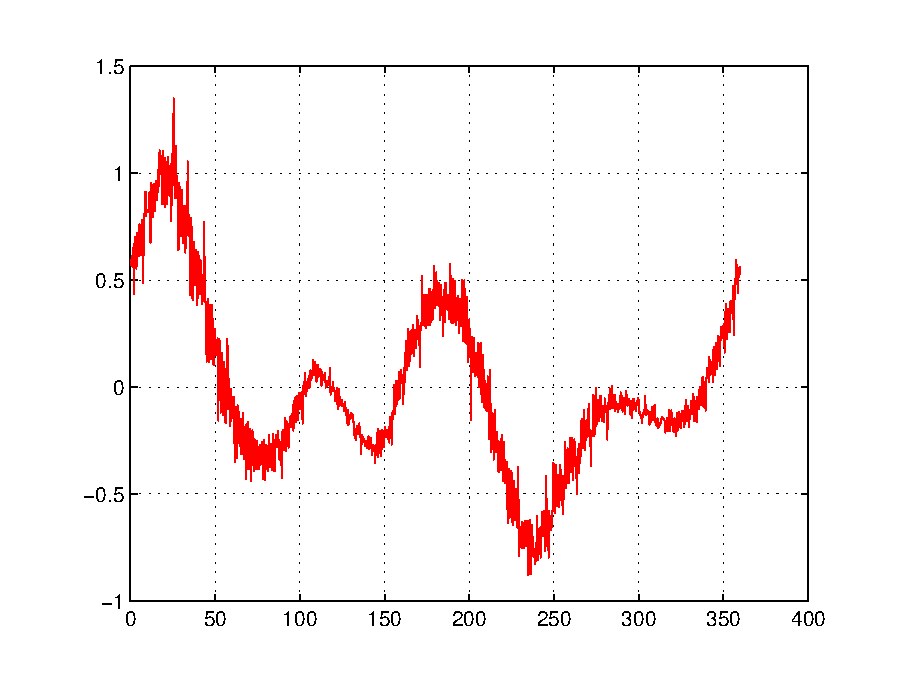
\includegraphics[scale=0.5]{\dirslike/protokol_meritve_ys_1.eps} % izpis_harmonikov.m
	\caption{Napaka pomerjenega kota pri stati"cni ekscentri"cnosti v y-osi}
	\label{fig:protokol_merjeni_ys_1}
\end{figure}




\begin{figure}[h!]
	
	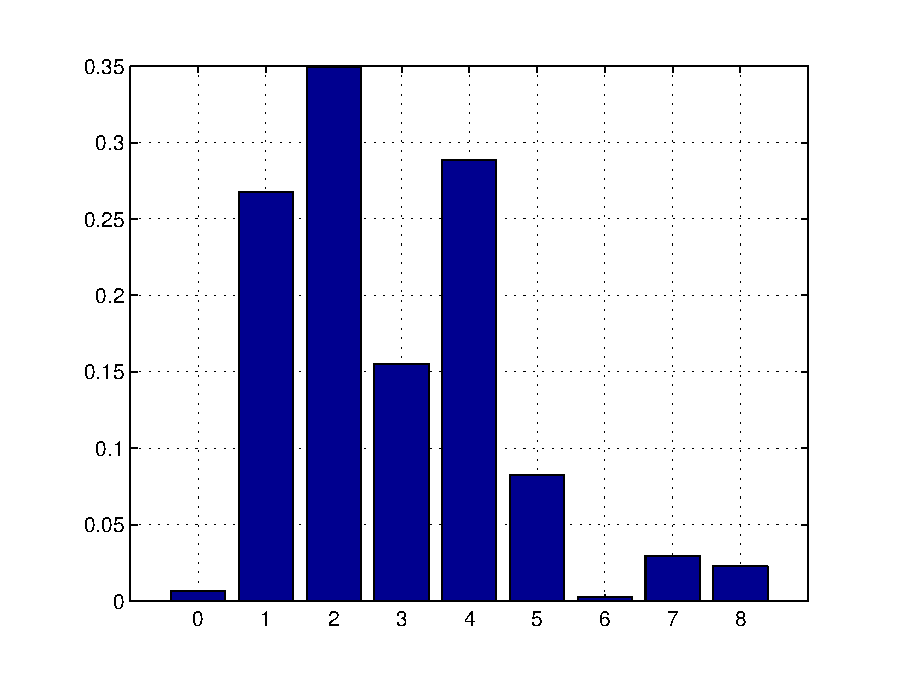
\includegraphics[scale=0.5]{\dirslike/vrsta_protokola_meritve_ys_1.eps} % izpis_harmonikov.m
	\caption{Razvoj napake v F vrsto pri stati"cni ekscentri"cnosti v y-osi}
	\label{fig:amplitude_merjeni__ys_1}
\end{figure}





\subsection{Napaka pri premiku senzorja v smeri z-osi}

V simulacijah tega dogodka nisme predvidel. Pri"cakoval bi, da se bo magnetno polje, ki ga pomerijo hallove sonde zmanj"salo. Tako bosta imela signala sinus in kosinus zmanj"sano amplitudo za enak faktor, kar na izra"cun kota ($\arctan$) ne bi imelo vpliva.
$$\arctan \frac{k \cdot y}{k \cdot x}=\arctan \frac{y}{x}$$
 Meritev je pokazala, da se ob premiku senzorja v z-osi pojavi napaka. Povi"sala se je amplituda prvega in tretjega harmonika.

\begin{figure}[h!]
	
	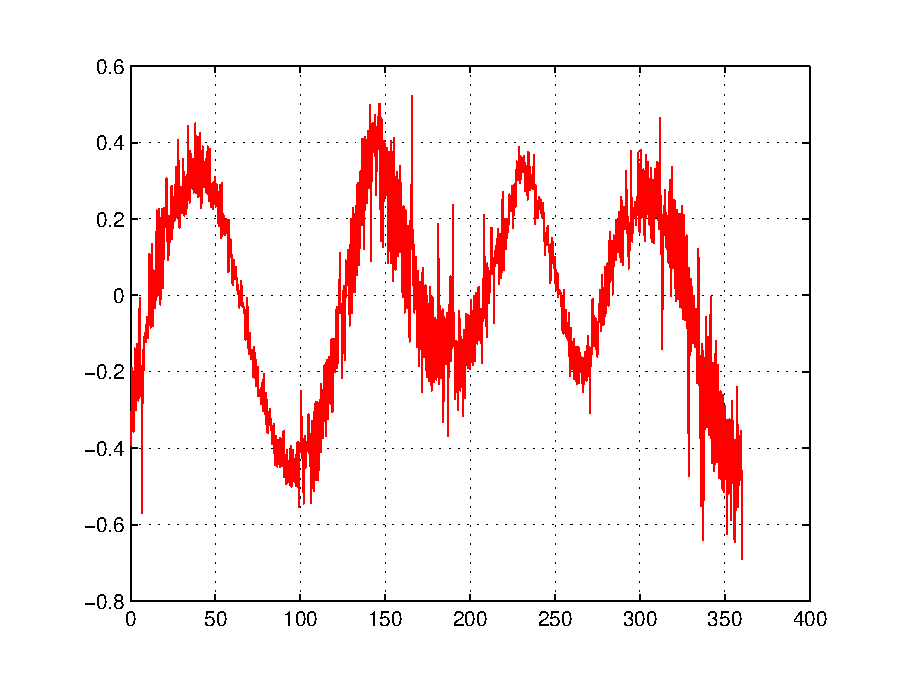
\includegraphics[scale=0.5]{\dirslike/protokol_meritve_zs_1.eps} % izpis_harmonikov.m
	\caption{Napaka pomerjenega kota pri stati"cni ekscentri"cnosti v z-osi}
	\label{fig:protokol_merjeni_zs_1}
\end{figure}




\begin{figure}[h!]
	
	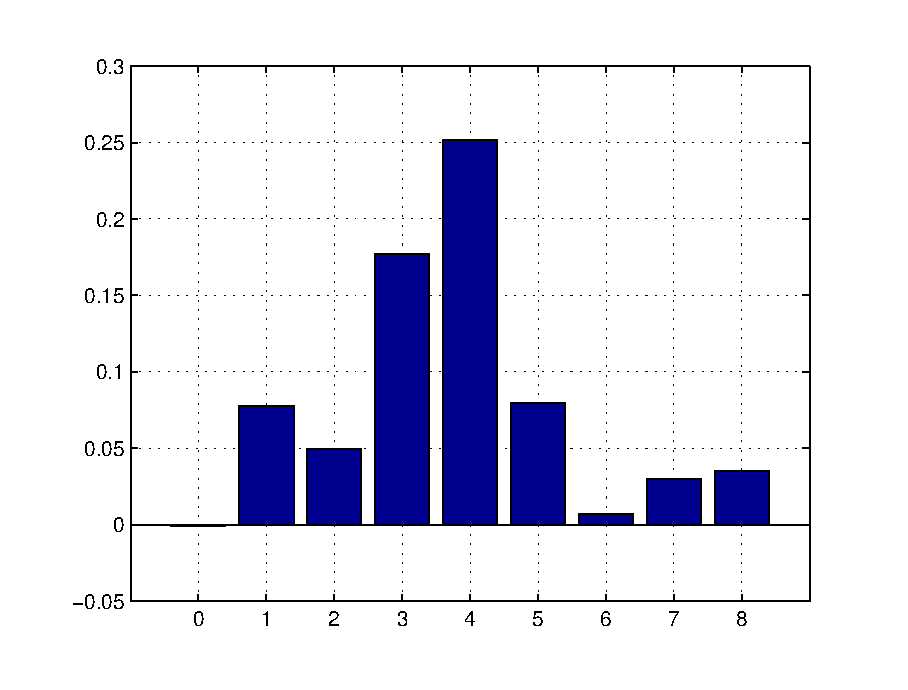
\includegraphics[scale=0.5]{\dirslike/vrsta_protokola_meritve_zs_1.eps} % izpis_harmonikov.m
	\caption{Razvoj napake v F vrsto pri stati"cni ekscentri"cnosti v z-osi}
	\label{fig:amplitude_merjeni__zs_1}
\end{figure}







\subsection{Napaka pri premiku magneta iz osi vrtenja}

Naparava omogo"ca premik magneta izven osi vrtenja le v eni smeri. Meritev je zato narejena le za en primer. Napaka je pomerjena pri premiku 125 $\mathrm{\mu m}$(Slika \ref{fig:protokol_merjeni__xd_1}). Opazi se, da se je pojavila napaka v obliki prvega harmonika. Z DFT-jem razvijemo napako na posamezne amplitude (Slika \ref{fig:amplitude_merjeni__xd_1}). Velikosti amplitud poka"zejo povi"sanje ammplitude prvega harmonika kar je bilo pri"cakovati. Spremenila se je tudi enosmerna komponeta napake.

\begin{figure}[h!]
	
	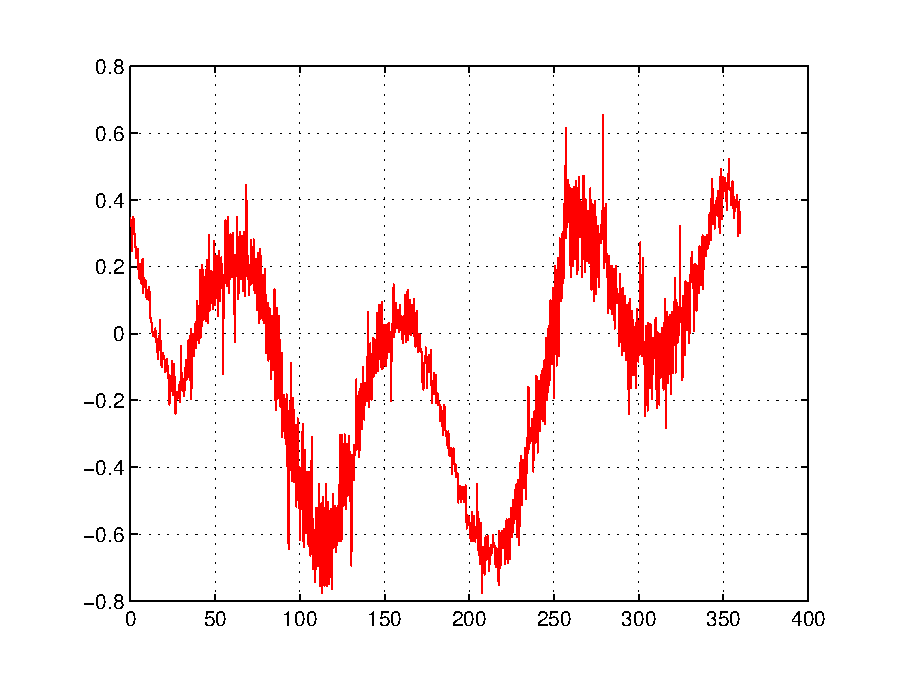
\includegraphics[scale=0.5]{\dirslike/protokol_meritve_xd_125.eps} % izpis_harmonikov.m
	\caption{Napaka pomerjenega kota pri dinami"cni ekscentri"cnosti 125u}
	\label{fig:protokol_merjeni_xd_1}
\end{figure}




\begin{figure}[h!]
	
	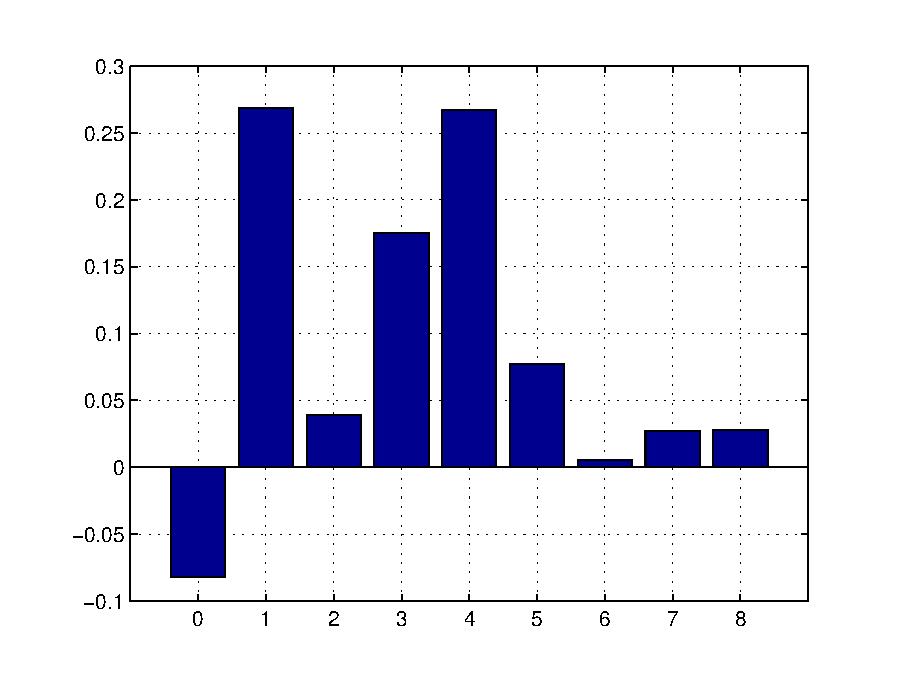
\includegraphics[scale=0.5]{\dirslike/vrsta_protokola_meritve_xd_125.eps} % izpis_harmonikov.m
	\caption{Razvoj napake v F vrsto pri dinami"cni ekscentri"cnosti 125u}
	\label{fig:amplitude_merjeni__xd_1}
\end{figure}

\subsection{Ve"canje stati"cne ekscentri"cnosti v x osi na napravi}

Kot v poglavju \ref{sec:vec_st_x}, sem tudi tu pomeril napako pri razli"cnih izmikih enkoderja iz idealne monta"ze. Napako sem z DFT-jem razstavil na posamezne harmonike. Na sliki \ref{fig:potek_amp_merjenih_xs}, so prikazani poteki spreminjanja velikosti posameznega harmonika napake v odvistnosti stati"cne ekscenri"cnosti v x-osi.

 
 \begin{figure}[h!]
 	
 	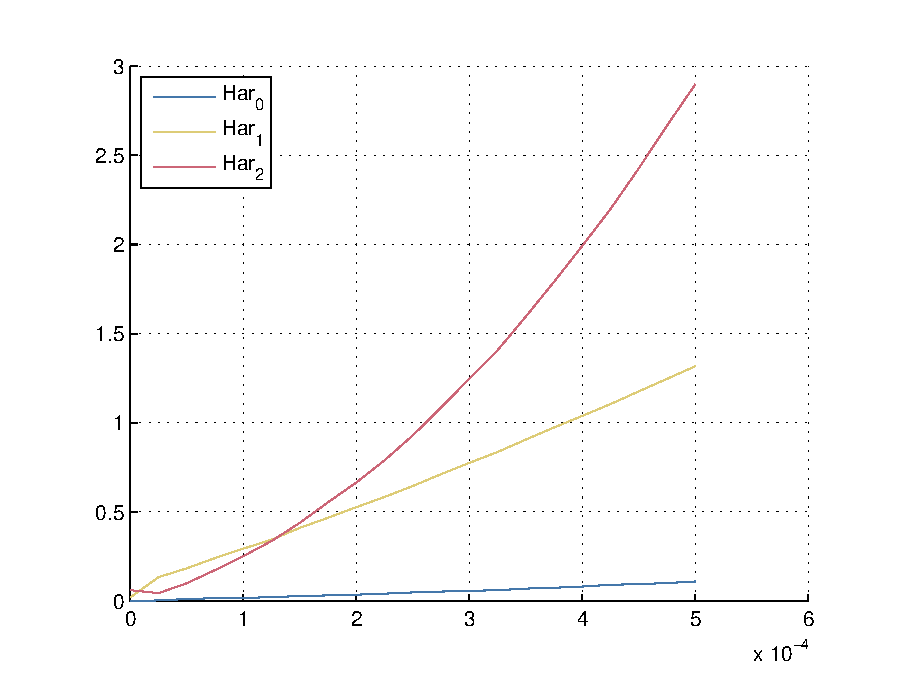
\includegraphics[scale=0.5]{\dirslike/potek_amp_merjenih_xs.eps} % izris_grafov_poteka_posameznih_amplitud.m folder='2017_09_27';	eksc='xs';	st_harmonikov=2;	periode=1;
 	\caption{Odvistnost posameznega harmonika napake od stati"cne ekscentri"cnosti v x osi}
 	\label{fig:potek_amp_merjenih_xs}
 \end{figure}

%delta x mora bit v milimetrih da bos popravil na vseh slikah
$A_0(\Delta x_s)=0.15740 \Delta x_s^3+0.01388 \Delta x_s^2+0.17182 \Delta x_s+0.00061$

$A_1(\Delta x_s)=1.81983 \Delta x_s^3-0.81049 \Delta x_s^2+2.49720 \Delta x_s+0.04854$

$A_2(\Delta x_s)=-1.75100 \Delta x_s^3+9.86952 \Delta x_s^2+1.23683 \Delta x_s+0.03126$




\appendix
Koeficienti ena"cbe (\ref{eq:polinom}):

\begin{align*}
a_1& = -3.613254883256721 \cdot 10^{-2}\\
a_2& = -9.397474474352774 \cdot 10^{-2}\\
a_3& =  2.270068566096036 \cdot 10^{-1}\\
a_4& = -1.654156805933996 \cdot 10^{-2}\\
a_5& =-1.412276545356571 \cdot 10^{-1}\\
a_6& =-8.091748555424770 \cdot 10^{0}\\
a_7& =-1.205821594072327 \cdot 10^{0}\\
a_8& =  3.574554554667357 \cdot 10^{-2}\\
a_9& =  4.384051669295653 \cdot 10^{1}\\
a_{10}& = 2.853582435899069 \cdot 10^{-1}
\end{align*}





\section{Brez ekscentri"cnosti}
 V ena"cbo (\ref{eq:polinom}), namesto x vstavimo izraz za $B_{H_1}$ iz ena"cbe (\ref{B_H_1_koncna}). Namesto y vstavimo izraz za $B_{H_2}$ iz ena"cbe (\ref{B_H_2_koncna}).
 Z upo"stevanjem, da ekscentri"cnosti ni, se izraza iz ena"cb (\ref{B_H_1_koncna}) in (\ref{B_H_2_koncna}) poenostavita v:
 
 \begin{equation}
 B_{H_1}=r_0 \cos(\theta)
 \end{equation}
 \begin{equation}
 B_{H_2}=r_0 \sin(\theta)
 \end{equation}
 
 Vstavimo izraza v (\ref{eq:polinom}) in poenostavimo.
 
\begin{equation}
\label{eq:brez_eks} 
\begin{split}
\varphi=0.2853582 + 0.1313764 r_0^2\\
-( 0.4544598 r_0 +0.0312348 r_0^3) \cos(\theta)\\
+ 0.0956307 r_0^2 \cos(2 \theta)\\
-0.0048977 r_0^3 \cos(3 \theta)\\
+(43.8404961 r_0- 0.9278593 r_0^3) \sin(\theta)\\
- 4.0458727 r_0^2 \sin(2 \theta)\\
+ 0.2779619 r_0^3 \sin(3 \theta)\\
 \end{split}
 \end{equation}
 
% "Ce za $r_0$ vzamemo $2.4$~mm se izraz (\ref{eq:brez_eks}) poenostavi v
 
% \begin{equation}
% \varphi=1.0313240 + 35.1223145\cdot \sin( \theta-2.484^\circ) - 
% 23.3193817\cdot\sin(2\cdot\theta+1.354^\circ) -3.8388171\cdot\sin(3 \cdot\theta-1.009^\circ)
% \end{equation}

\section{Staticna ekscentri"cnost v x-osi}

V izrazih (\ref{B_H_1_koncna}) in (\ref{B_H_2_koncna}) upo"stevamo, da je stati"cni izmik v x-osi. $\Delta x_s$ ni 0, $\Delta y_s$ in $\Delta x_d$ sta 0 in izraza za $B_{H_1}$ in $B_{H_2}$ sta enaka:


\begin{equation}
\label{B_H_1_xs}
B_{H_1}=(r_0+\Delta x_s) \cos(\theta)
\end{equation}

\begin{equation}
\label{B_H_2_xs}
B_{H_2}=\Delta x_s \cos(\theta)+r_0 \sin(\theta)
\end{equation}

Vstavimo v (\ref{eq:polinom}) in dobimo:


\begin{equation}
\label{eq:eks_xs_analiticno} 
\begin{split}
\varphi=
0.2853582 + 0.1313764 r_0^2 - 3.8188667 r_0 x_s -3.9144993 x_s^2\\
 + (-0.0312348 r_0^3 + 43.3860817 x_s -1.0602813 r_0^2 x_s \\- 1.0143530 x_s^3 
+r_0 (-0.4544598 - 0.2346663 x_s^2)) \cos[\theta]\\
 + (0.0956307 r_0^2 - 3.8188667 r_0 x_s - 3.9144993 x_s^2) \cos[2 \theta] \\
+(-0.0048977 r_0^3 + 0.8579069 r_0^2 x_s - 
0.0782219 r_0 x_s^2 - 0.3381179 x_s^3) \cos[3 \theta] \\
+r_0 (43.8404961 - 0.9278593 r_0^2 - 0.0552582 r_0 x_s - 
0.0552582 x_s^2)\sin[\theta]\\
 + r_0(-4.0458841 r_0 - 4.0101318 x_s)  \sin[2\theta]\\
+r_0 (0.2779619 r_0^2 - 0.0552582 r_0 x_s - 0.9361328 x_s^2) \sin[3 \theta]
\end{split}
\end{equation}



\section{Staticna ekscentri"cnost v y-osi}

V izrazih (\ref{B_H_1_koncna}) in (\ref{B_H_2_koncna}) upo"stevamo, da je stati"cni izmik v y-osi. $\Delta y_s$ ni 0, $\Delta x_s$ in $\Delta x_d$ sta 0 in izraza za $B_{H_1}$ in $B_{H_2}$ sta enaka:





\begin{equation}
\label{B_H_1_ys}
B_{H_1}=r_0 \cos(\theta)+\Delta y_s \sin(\theta)
\end{equation}

\begin{equation}
\label{B_H_2_ys}
B_{H_2}=(r_0+\Delta y_s) \sin(\theta)
\end{equation}


Vstavimo v (\ref{eq:polinom}) in dobimo:


\begin{equation}
\label{eq:eks_ys_analiticno} 
\begin{split}
\varphi=
0.2853582 + 0.1313764 r_0^2 -  4.0101261 r_0 y_s - 
3.9144993 y_s^2 \\
+r_0  (-0.4544598 - 0.0312348 r_0^2 - 0.0552582 r_0 y_s - 
0.0782219 y_s^2 )\cos(\theta)\\
+ (0.0956307 r_0^2 + 4.0101261 r_0 y_s + 
3.9144993 y_s^2) \cos(2 \theta)\\
+(- 0.0048977 r_0^3 + 
0.0552582 r_0^2 y_s + 0.0782219 r_0 y_s^2) \cos(3 \theta)\\
+(43.8404961 r_0  - 0.9278593 r_0^3+43.3860817 y_s  - 2.7760952 r_0^2 y_s\\
 -2.8083928 r_0 y_s^2  - 1.0143530 y_s^3) \sin(\theta)\\
+r_0  (-4.0458841 r_0 - 3.8188784 y_s) \sin(2 \theta)\\
+(0.2779619 r_0^3 + 0.8579069 r_0^2 y_s  + 
0.9361328 r_0 y_s^2  + 0.3381179 y_s^3 )\sin(3 \theta)\\
\end{split}
\end{equation}











\section{Dinami"cna ekscentri"cnost v x-osi}

V izrazih (\ref{B_H_1_koncna}) in (\ref{B_H_2_koncna}) upo"stevamo, da je stati"cni izmik v x-osi. $\Delta x_d$ ni 0, $\Delta x_s$ in $\Delta y_s$ sta 0 in izraza za $B_{H_1}$ in $B_{H_2}$ sta enaka:





\begin{equation}
\label{B_H_1_xd}
B_{H_1}=r_0 \cos(\theta)-\Delta x_d
\end{equation}

\begin{equation}
\label{B_H_2_xd}
B_{H_2}=r_0 \sin(\theta)-\Delta x_d
\end{equation}


Vstavimo v (\ref{eq:polinom}) in dobimo:


\begin{equation}
\label{eq:eks_xd_analiticno} 
\begin{split}
\varphi=
0.2853582 + 0.1313764 r_0^2 - 43.3860817 x_d\\
 + 1.9181882 r_0^2 x_d -  7.8290100 x_d^2 + 1.3524727 x_d^3\\ 
+(- 0.4544598 r_0
- 0.0312348 r_0^3  + 7.6377568 r_0 x_d 
- 0.3128888 r_0 x_d^2) \cos(\theta)\\
 + (0.0956307 r_0^2  
- 1.7158195 r_0^2 x_d) \cos(2 \theta)\\
 - 0.0048977 r_0^3 \cos(3 \theta)\\
+ (43.8404961 r_0  - 0.9278593 r_0^3 
+ 8.0202637 r_0 x_d - 3.7445199 r_0 x_d^2) \sin(\theta) \\
+(- 4.0458727 r_0^2  + 0.1105161 r_0^2 x_d) \sin(2 \theta)\\ 
+ 0.2779619 r_0^3 \sin(3 \theta)
\end{split}
\end{equation}


%\section{Dolo"canje kota pri stati"cni ekscntri"cnosti v smeri y }
%\begin{equation}
%\varphi=\frac{(r_0+\Delta y_s)\sin(\theta) (8 r_0^2+4r_0 \Delta y_s + 8 \Delta y_s^2)\cos (2 \theta) +12 r_0 \Delta y_s \sin (2 \theta)}
%{((3 r_0^3  +3 r_0 \Delta y_s^2) \cos(\theta) + (r_0^3-3r_0 \Delta y_s) \cos(3 \theta )+ (3 r_0^2 \Delta y_s+3\Delta y_s^3)\sin(\theta)+(3 r_0^2 \Delta y_s - \Delta y_s^3)\sin(\theta))}
%\end{equation}
%
%

%\begin{figure}
%\centering
%\begin{tikzpicture}[scale=1]
%\magnet {0} {0} {10}{ }{1}
%\senzorja{0}{0.5}{0}{$S_h$}
%\draw (0,0) circle (0.5);
%\senzorja{-0.35}{0.35}{45}{$S_h$}


%\end{tikzpicture}
%\caption{Prikaz navora v odvistnosti od komponent toka }
%
%\label{fig:navor}
%\end{figure}
%izpeljava ekscentricnosti za 1 senzor [x0,y0]

%\section{izpeljava stati"cne ekscentri"cnosti}
%Napises da je senzor izmaknjen iz centra magneta in sredisce senzorja opise kroznico
%
%
%
%
%\section{izpeljava dinami"cne ekscentri"cnosti}
%napisi da je magnet izmaknjen senzor pa zavrtis okoli sredisca senzorja






%\section{Rezultati simulacij}
%
%\chapter{Zaklju�ek} \label{zakljucek}
%
%
%


\end{document}
